\chapter{Introduction} \label{cpt-introduction}

Ever since the early days of computer graphics, both hardware and software have rapidly evolved
alongside the creative and challenging use cases provided by developers, scientists, and others.
Many technical increments relied on innovation, especially the advent of new capable hardware.
One example is the \ac{GPU} itself, which is now considered the heart of modern graphics 
processing and is widely used in fields like science, artificial intelligence, games, and pretty 
much all graphics-related applications. \\

\noindent
The year 2024 marks the 25th anniversary of what is considered to be the first consumer grade PC 
\ac{GPU}, the \emph{NVIDIA GeForce 256}. Although graphics chips had been around for a while, 
especially in the professional space of the industry, this card was the first to be marketed 
as a \ac{GPU}. 

\begin{quote}
    "\emph{What makes the GeForce different than its predecessors is the chip's ability to take over all 
    processing functions for creating three-dimensional graphics. Previously, the computer's main 
    processor would have to share in that responsibility, which could result in slower load times 
    and 'stuttering' on the part of the software.}" \\  
    (CNN Money \cite{CNNMoney1999}, 1999)
\end{quote}

\noindent
Before 1999, the graphics units were specialized chips either used for video encoding and decoding
or expensive hardware targeted for large companies, which arised during the early stages of "3D 
consumer graphics" \cite{Singer2023}. Dedicated and affordable \ac{GPU}s for consumer \ac{PC} had 
their large breakthrough during the 1990s. With the introduction of the \emph{NVIDIA GeForce 256}, 
efficient transformations and lighting computations found their way into private \ac{PC}s 
\cite{Fenno2024}. Back then, this new hardware created a multitude of new possibilities. Some of the 
major innovations featured \emph{cube mapping}, \emph{per-pixel light calculations}, and a 
\emph{standardized vertex buffer} \cite{NVIDIA1999, Battaglia2024}. [@TODO: Re-check vertex buffer] \\

\noindent
Although it was mostly used for graphics processing - hence the name - nowadays, \ac{GPU}s are used 
in a much more general way than in 1999. Both the technical complexity and the fields of application 
have tremendously increased. Today, a \ac{GPU} is often referred to as a \ac{GPGPU} because of its 
evolution towards a multi-purpose tool. \\

\noindent
Nevertheless, \ac{GPU} architecture is still under a strong influence of the entertainment 
industry, first and foremost the games industry. Some of the latest changes to \ac{GPU} 
hardware and \ac{API} design correlate to the ongoing demand for higher output resolutions, 
higher geometric density, and additionaly technology for \emph{Deep Learning} algorithms. 
These possibilities led to a lot more applications of \ac{GPU}s in various fields of science, 
like biology, machine learning, video encoding and decoding, and more \cite{Battaglia2024}.
To provide more context for how some of the more modern features of \ac{GPU}s can be of great 
use for new software approaches, a brief overview over the trends in computer graphics over 
the past decades, and especially the last years, is given.


\section{Evolution of Real-Time-Rendering} \label{sec-evolution-of-real-time-rendering}
[@TODO: double check games]

\begin{figure}[h]
    \centering
    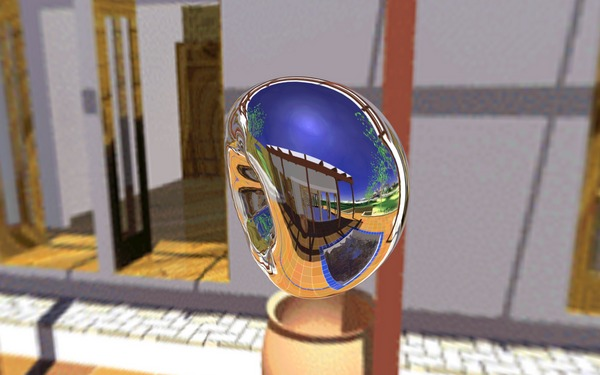
\includegraphics[width=250px]{images/graphics/bubble-reflection-effects-demo.jpg}
    \caption{The \emph{NVIDIA} bubble demo showcasing advanced reflections using cube mapping (\emph{NVIDIA} \cite{NVIDIABubble}, 2000).}
    \label{fig:bubble-reflection-demo}
\end{figure}

\noindent
Before the integration of specialized hardware, games like \emph{Wolfenstein 3D} or the 
original \emph{Doom} made heavy use of \ac{CPU} computations for graphics processing, 
executed sequentially \cite{NVIDIA1999}. A major problem was the demand for increasing 
visual fidelity. Games needed to get bigger, more photorealistic, and provide more dense 
geometry. Increasing the amount of triangles rendered ultimately led to worse runtime 
performance. The advent of a dedicated, massively parallel chip to perform a large amount of 
operations introduced a solution for this problem. Over the years, more and more stages of the 
rendering pipeline were offloaded to the \ac{GPU}, which in turn resulted in a lot of new effects, 
games with higher triangle density and new lighting technology. As mentioned before, the \emph{NVIDIA 
GeForce 256} introduced cube mapping to the pipeline featuring real-time reflections, which is 
shown in Figure \ref{fig:bubble-reflection-demo} \cite{Battaglia2024}.


\subsection*{Rendering Pipeline} \label{subsec-rendering-pipeline}

The standardization of the graphics hardware, as pioneered by \emph{NVIDIA}, in concert with capable 
graphics \ac{API}s like \emph{Direct3D} or \emph{OpenGL} kick-started huge graphical improvements in 
games and computer graphics. The heavily parallelized transformations allowed for a lot more triangles 
in games, and the hardware-accelerated lighting computations made for even more realistic lighting 
throughout the rendered scenes. One significant advantage: The \ac{GPU} could operate on a large amount 
of data while not stalling the \ac{CPU} \cite{Fenno2024}.\\

\noindent
The new rendering pipeline was to be seen in a lot of games, some of the first being \emph{Epic Games'} 
\emph{Unreal Turnament} (1999) and \emph{id Software's} \emph{Quake III Arena} (1999) \cite{UnrealTurnament, 
Quake3Arena}. \emph{Microsoft's} multimedia \ac{API} \emph{DirectX 7} added support for the new \ac{TL} 
features of \ac{GPU}s. During the following years, more and more features were added, slowly evolving the 
standard towards the "modern" rendering pipeline that is used nowadays. Between the years 1999 and 2009,
20 new minor versions of \emph{DirectX} were released \cite{WikiDirectX}.

\begin{figure}[h]
    \centering
    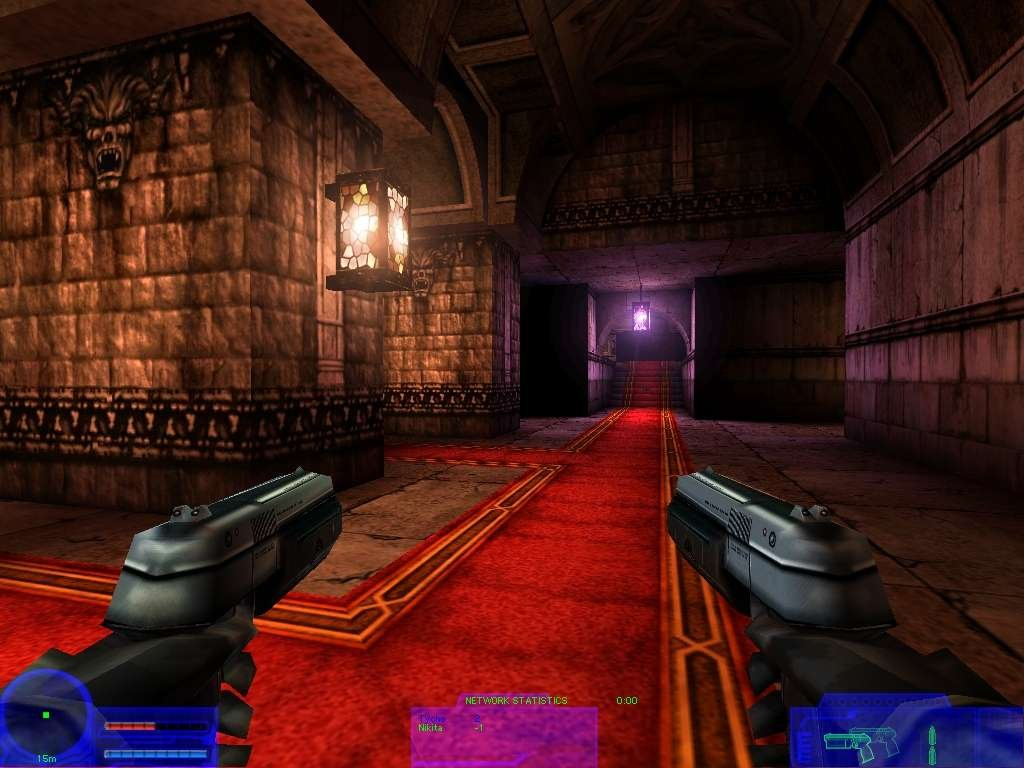
\includegraphics[width=172.5px]{images/graphics/unreal-turnament.jpg}
    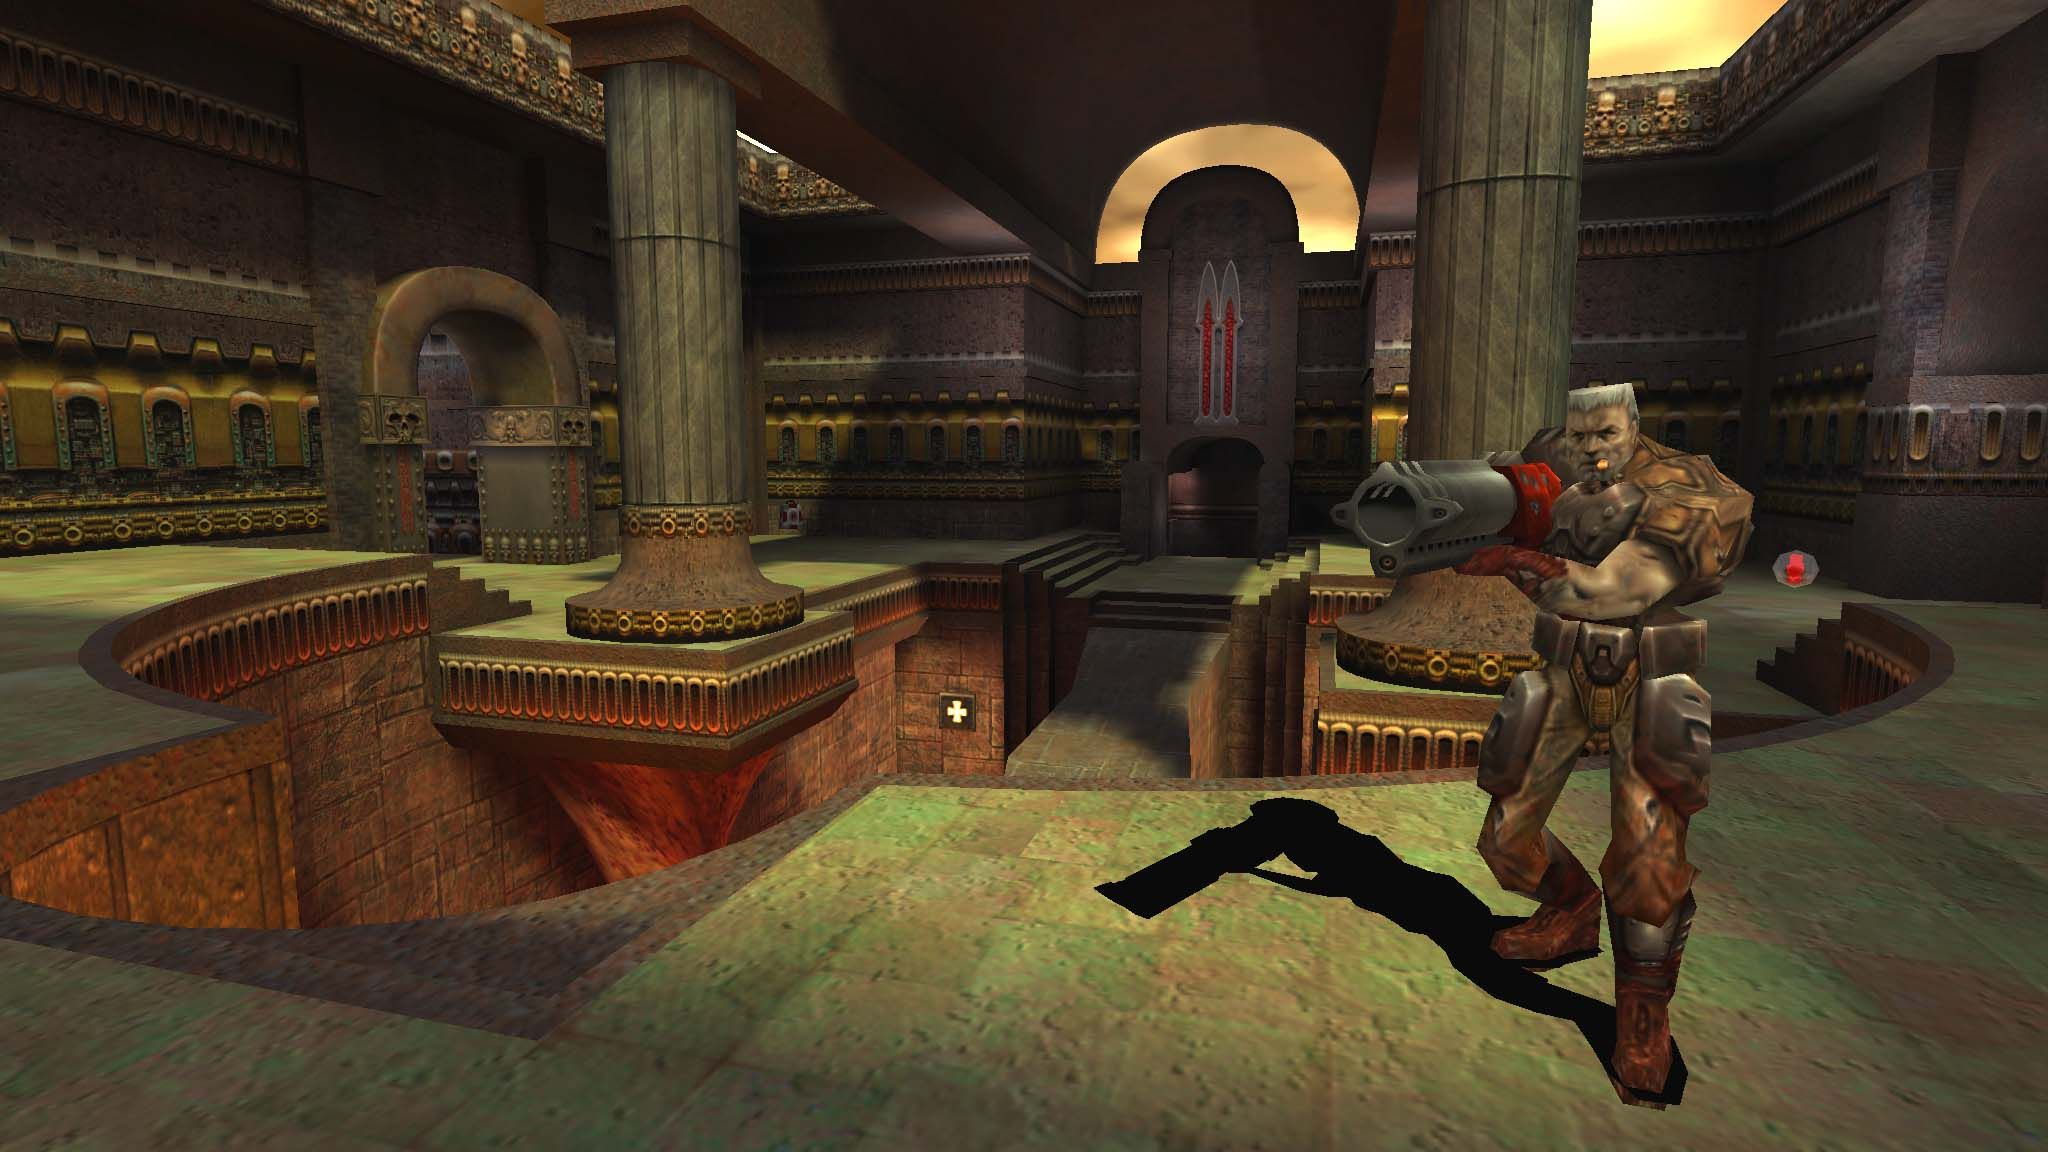
\includegraphics[width=230px]{images/graphics/quake-iii-arena.jpg}
    \caption{A screenshot from the game \emph{Unreal Turnament} (1999) (left) and \emph{Quake III Arena} (1999) 
    (right) \cite{GamespotUnrealTurnament, GameWatcher2006}.}
    \label{fig:unreal-turnament-quake-arena}
\end{figure}


\subsection*{Programmable Pipeline Stages}
 
One of the first steps to integrating advanced per-pixel operations into the pipeline was the combination of
multiple textures for use on the same fragment. This soon evolved to become more potent when \emph{NVIDIA} 
introduced the \emph{GeForce 3} graphics card, which "contained the first example of true programmability" 
\cite{KhronosProgramibility2024}. A specific vertex processor, equipped with 256 4-vector uniforms, was 
introduced to execute custom operations on vertices. The same trend was seen in the per-pixel operations, 
which also became its own programmable stage \cite{KhronosProgramibility2024}. \\

\begin{figure}[h]
    \centering
    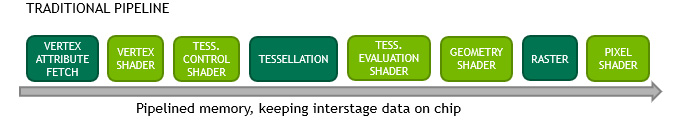
\includegraphics[width=\linewidth]{images/graphics/traditional-rendering-pipeline.jpg}
    \caption{The rendering pipeline and its stages. The stages colored in light green are programmable, 
    the ones colored in dark green are configurable \cite{Kubisch2018}.}
    \label{fig:traditional-rendering-pipeline}
\end{figure}

\noindent
The programmability of the stages enabled developers to customize their applications and the output presented 
on screen. It also contributed to a more parallelized architecture, which improved computation capabilities on 
the \ac{GPU} instead of sequential computations by the \ac{CPU}. Over the years, more stages like the 
\emph{Geometry Shader} stage were added, and the stages were expanded to be programmable - or at least configurable. \\

\noindent
Today, this is still considered the "standard rendering pipeline", although current advances in hardware and software 
introduced additions to the pipeline or even offered replacement technology for computing three-dimensional data.
Nevertheless, these new innovations increase the programmability and customization capabilities of the pipeline,   
following a trend that began decades ago.


\subsection*{Deferred Shading} \label{subsec-deferred-rendering}

With a lot of innovative hardware and software, the games got more complex, and real-time computer graphics got even 
more photorealistic. The demand for more light sources increased in an attempt to make game worlds more realistic. 
However, more light sources posed some problems for the developers. When using the traditional rendering pipeline, 
lighting is calculated on a per-vertex basis. Interpolation can be used to generate lighting results for every sample 
in between the vertices. Still, every vertex must be considered in combination with all light sources. This creates a 
dependancy between the number of vertices and the number of lightsources. Basically, adding a few more light sources 
will drastically increase the computation times of the final image. \\

\noindent
To improve this, another method was adopted: \emph{Deferred Shading}. It was first adopted for the use on \ac{GPU}s 
by Dean Calver \cite{Calver2004} in 2004. This technique makes use of multiple render targets and writes the data 
necessary for the lighting calculations into various buffers. This way, the surface normals, the specular intensity, 
the albedo (texture color), the depth and more values can all be stored individually, as per-pixel data. This includes 
the relevant data for the lighting calculations. When all buffers are drawn, the final result is easily found by 
looking up all the relevant data from each buffer at one pixel coordinate and combining them to a final result. 
Figure \ref{fig:deferred-shading-buffers} shows an example of all the buffers used for the creation of one frame in 
\emph{Guerilla Games'} \emph{Killzone 2} (2009) \cite{KillzoneFandom}. 

\begin{figure}[!]
    \centering
    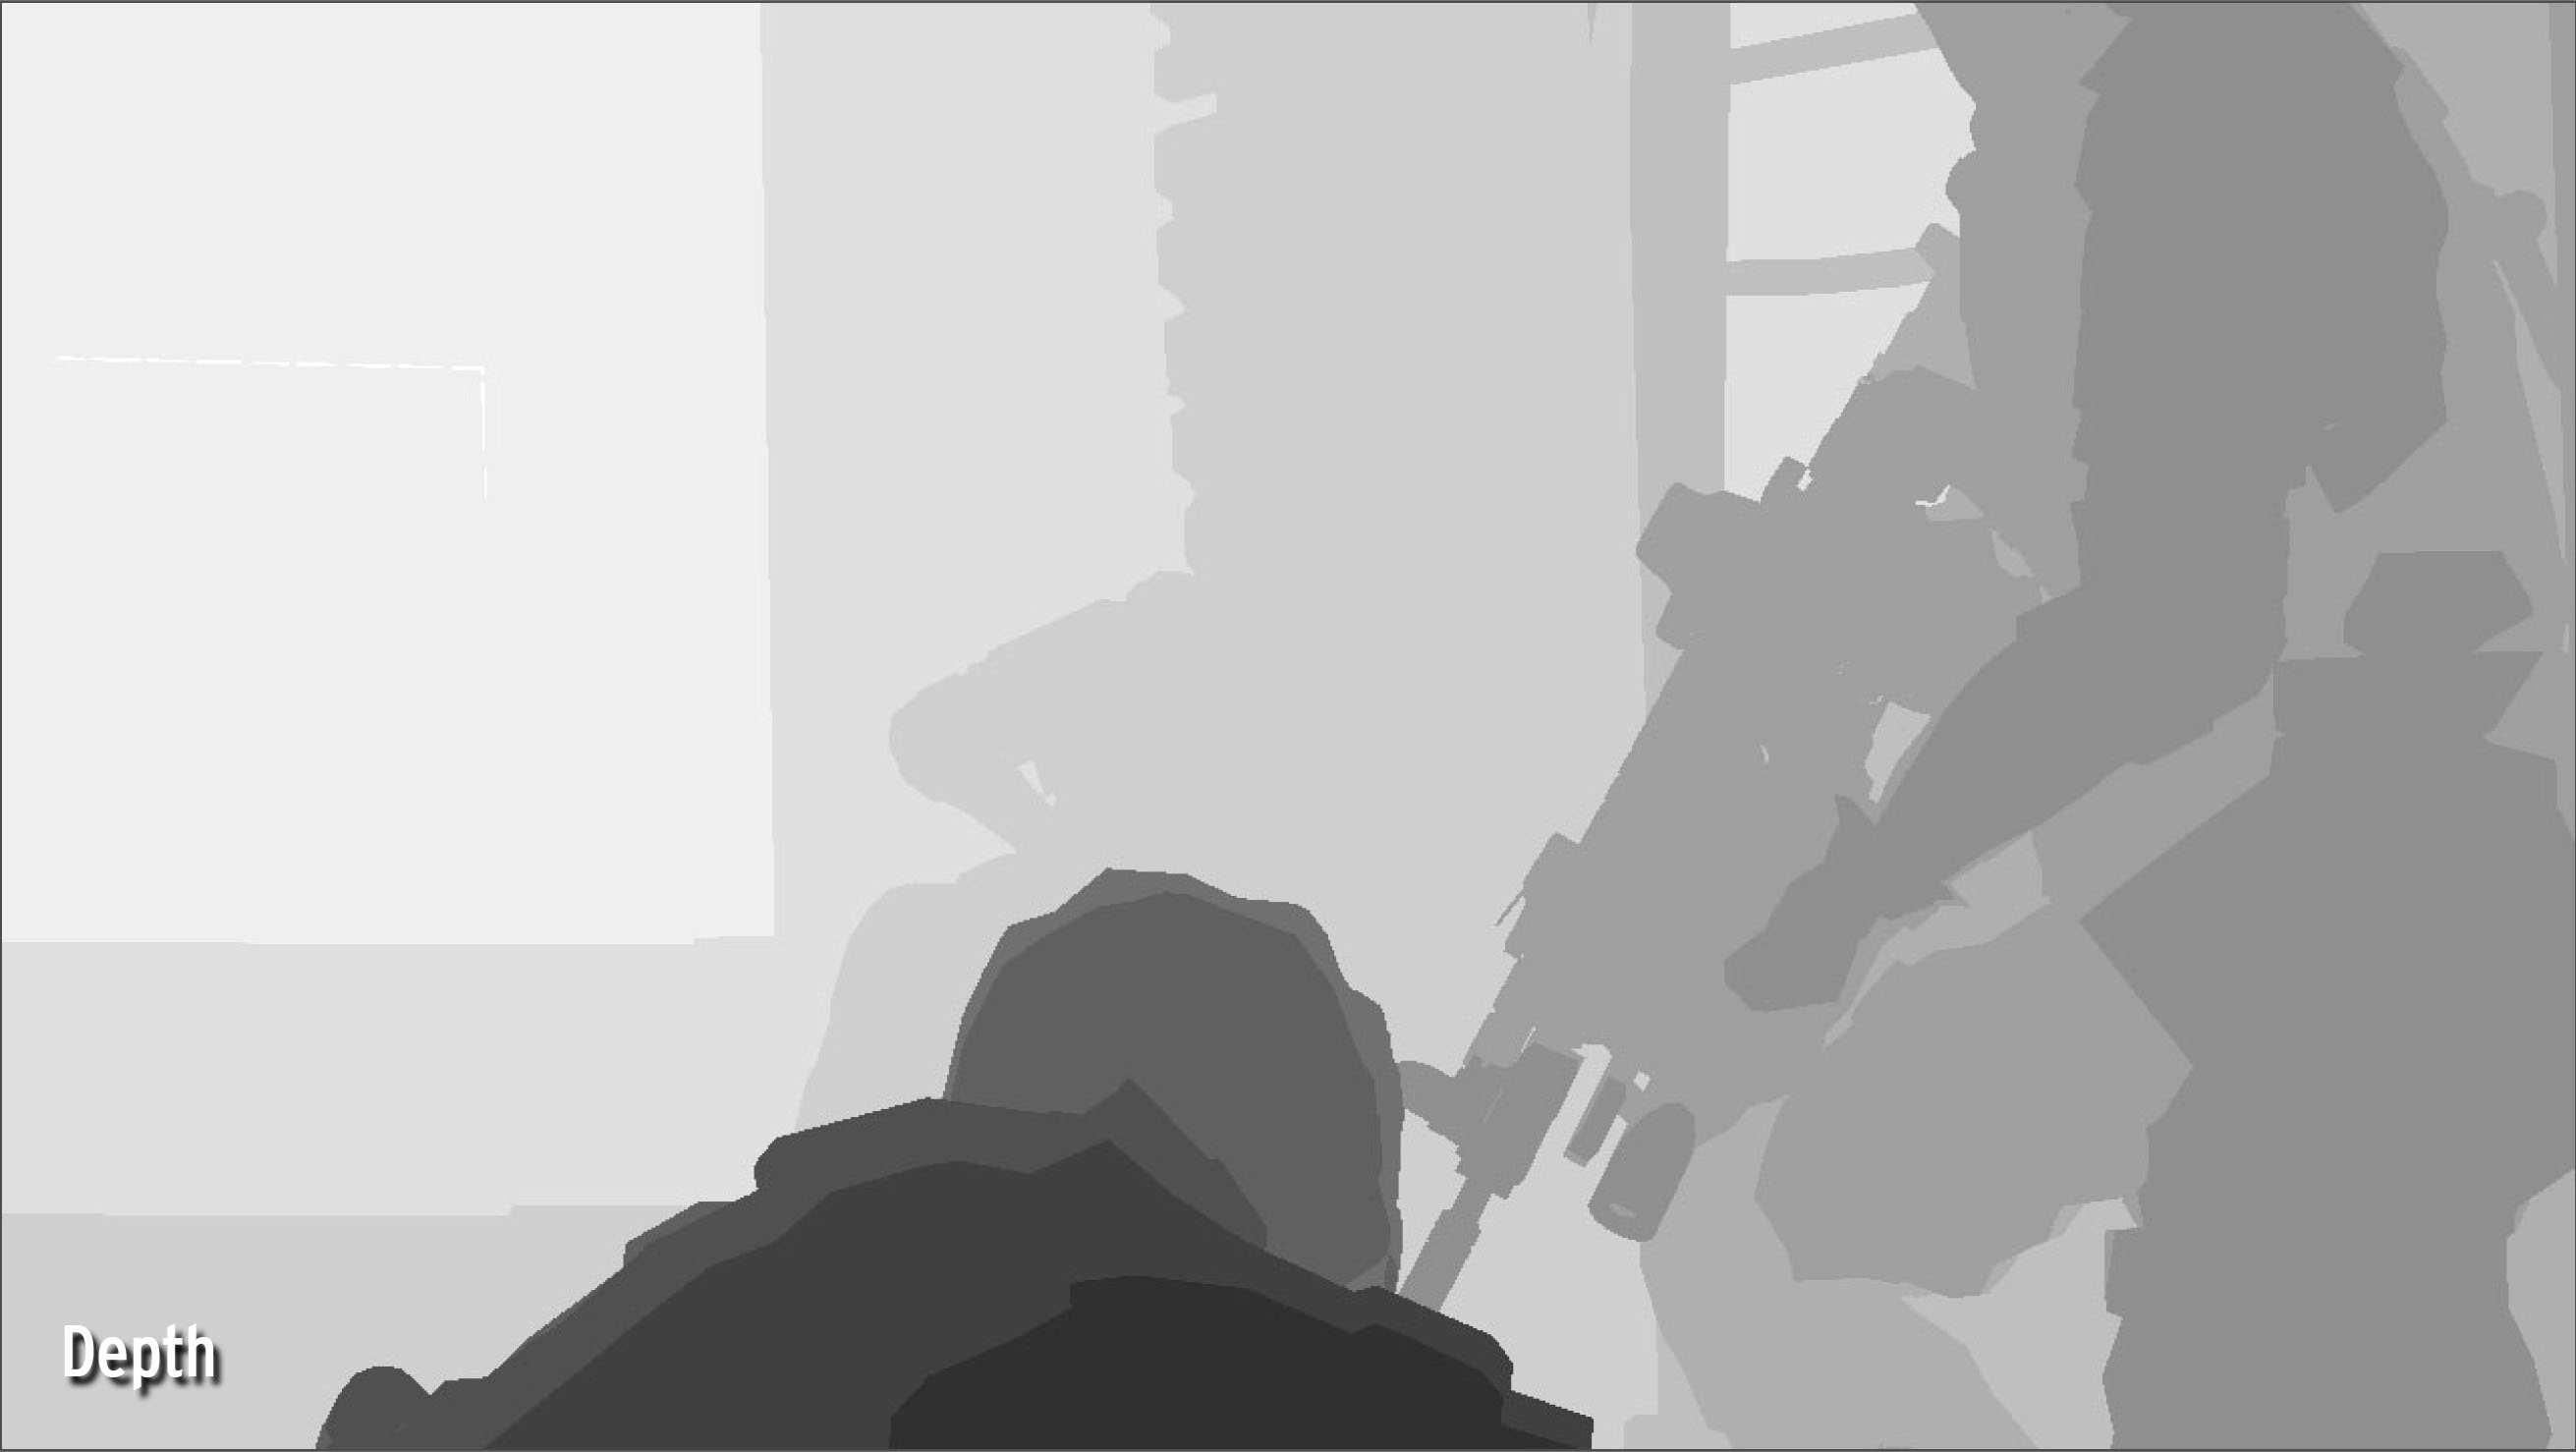
\includegraphics[width=175px]{images/graphics/killzone-2-buffer-depth.jpg}
    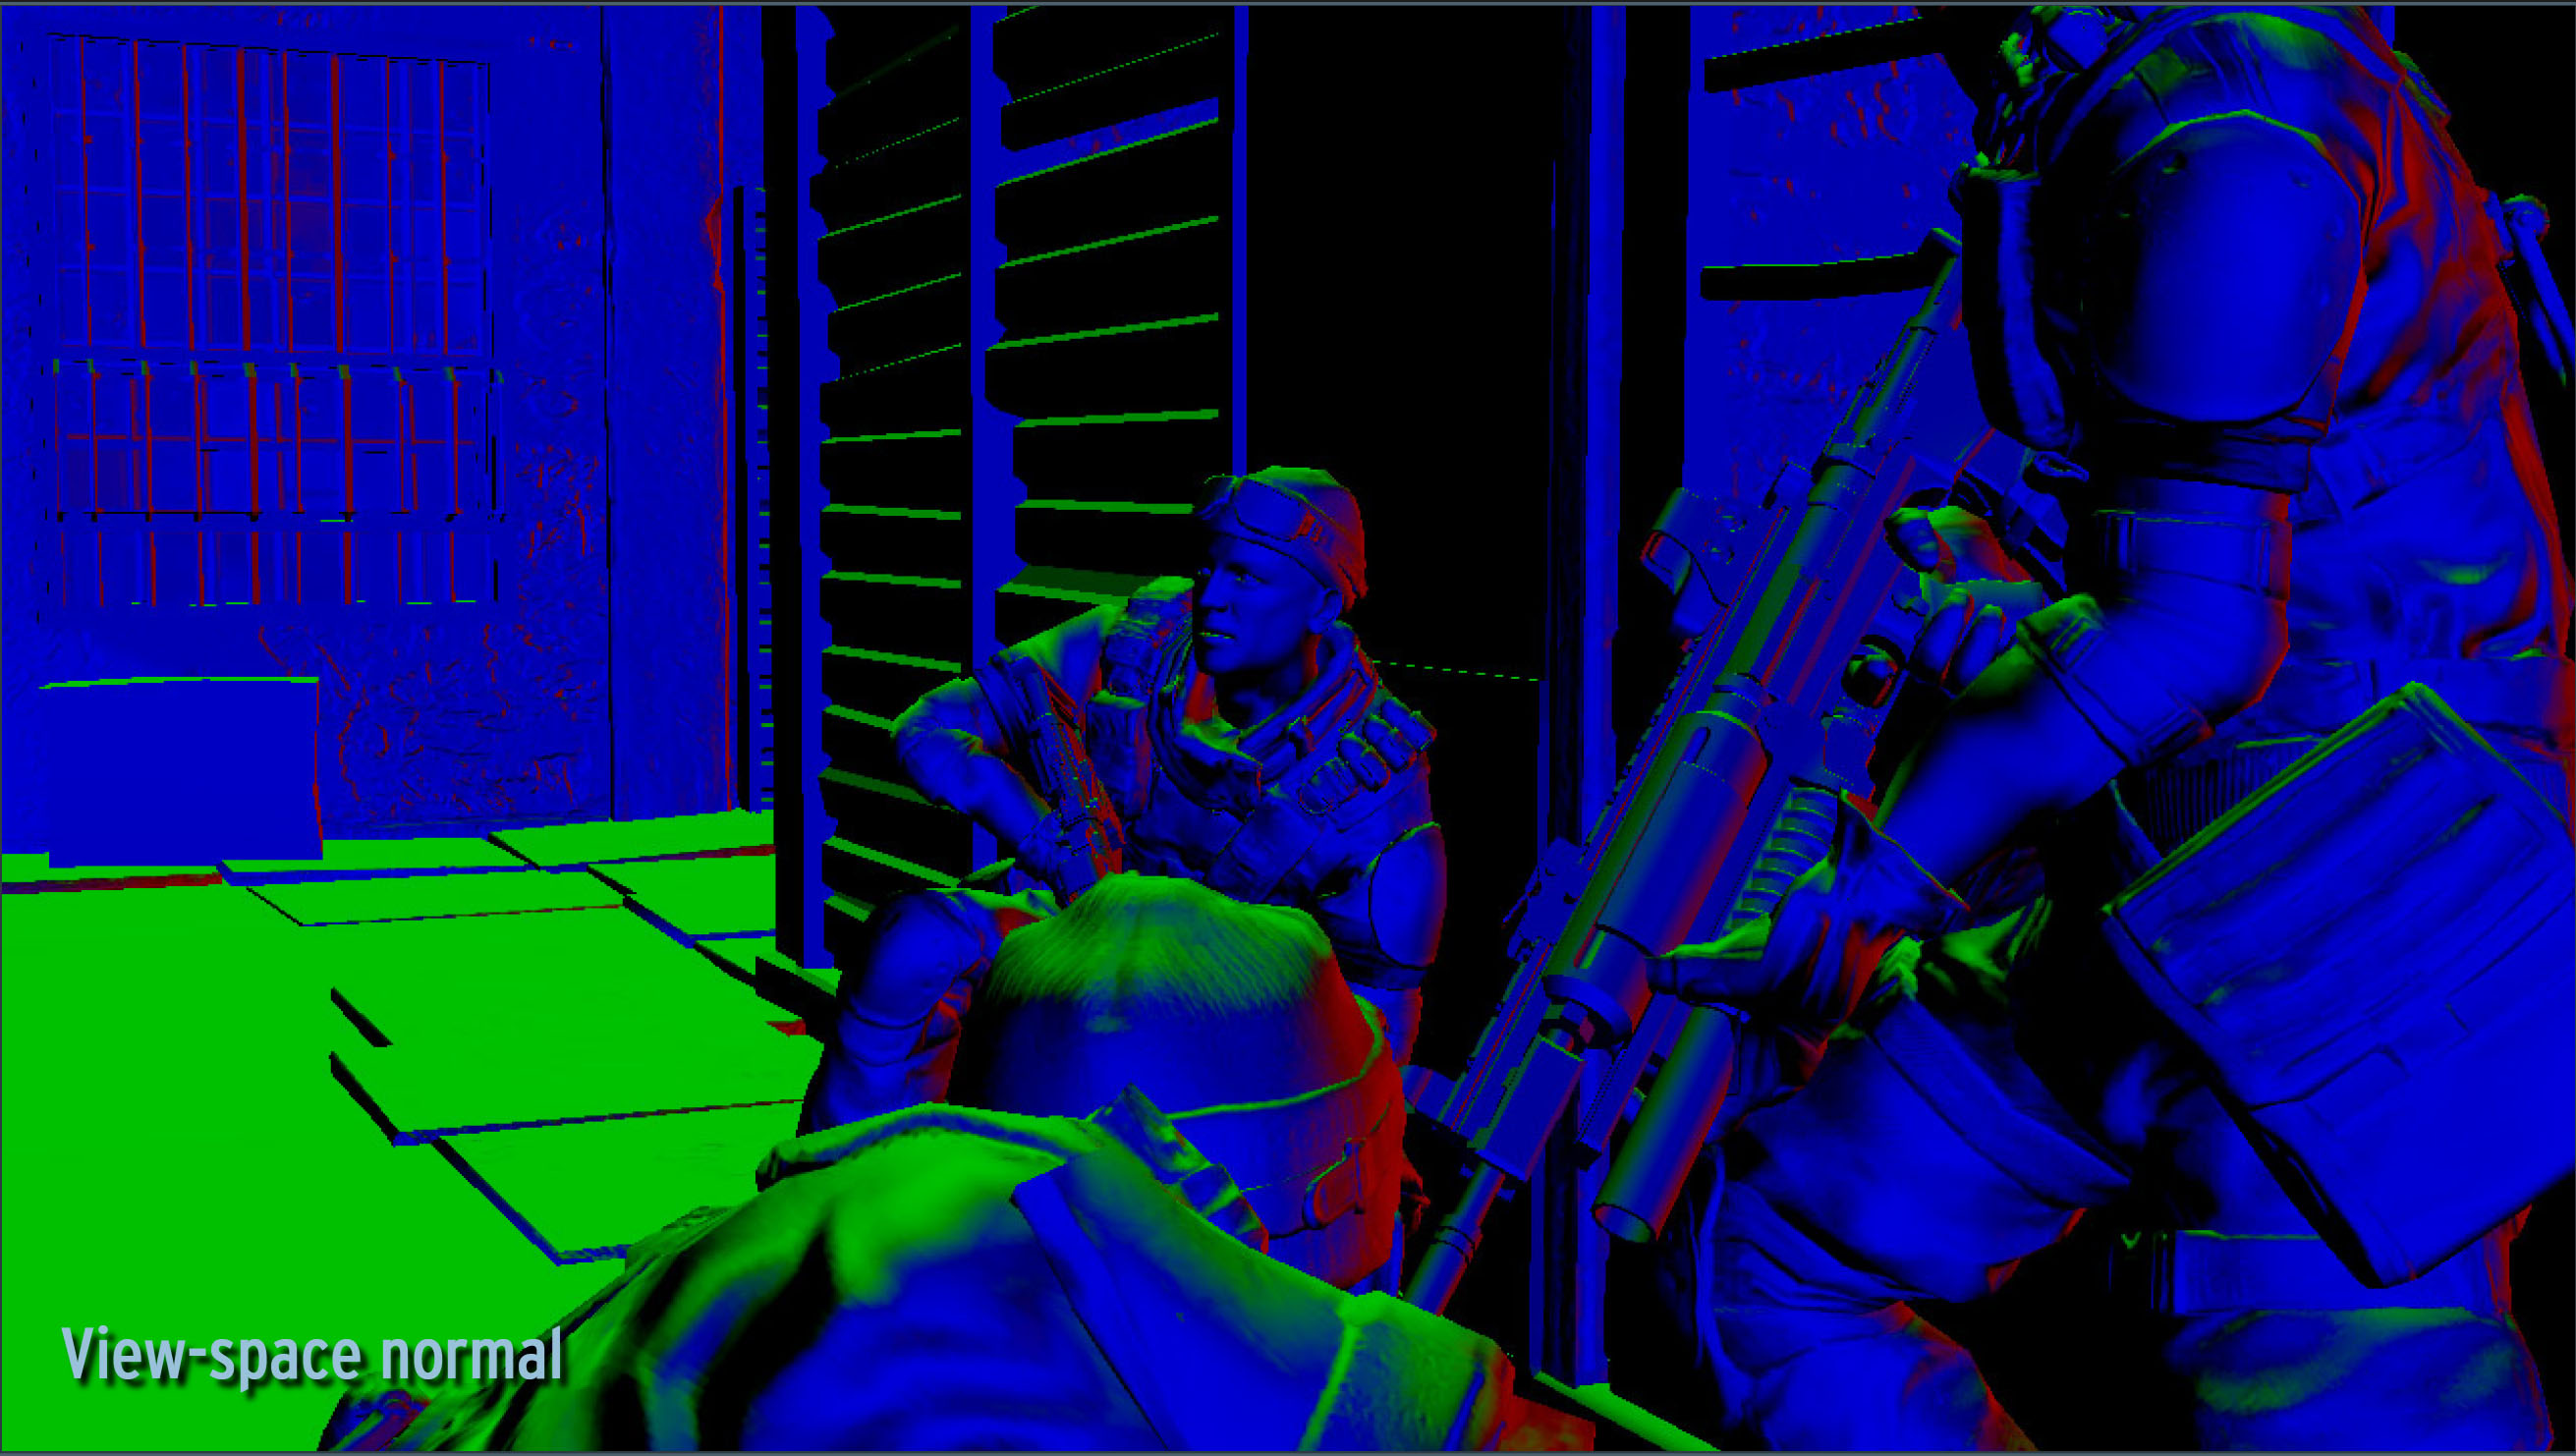
\includegraphics[width=175px]{images/graphics/killzone-2-buffer-vsn.jpg}
    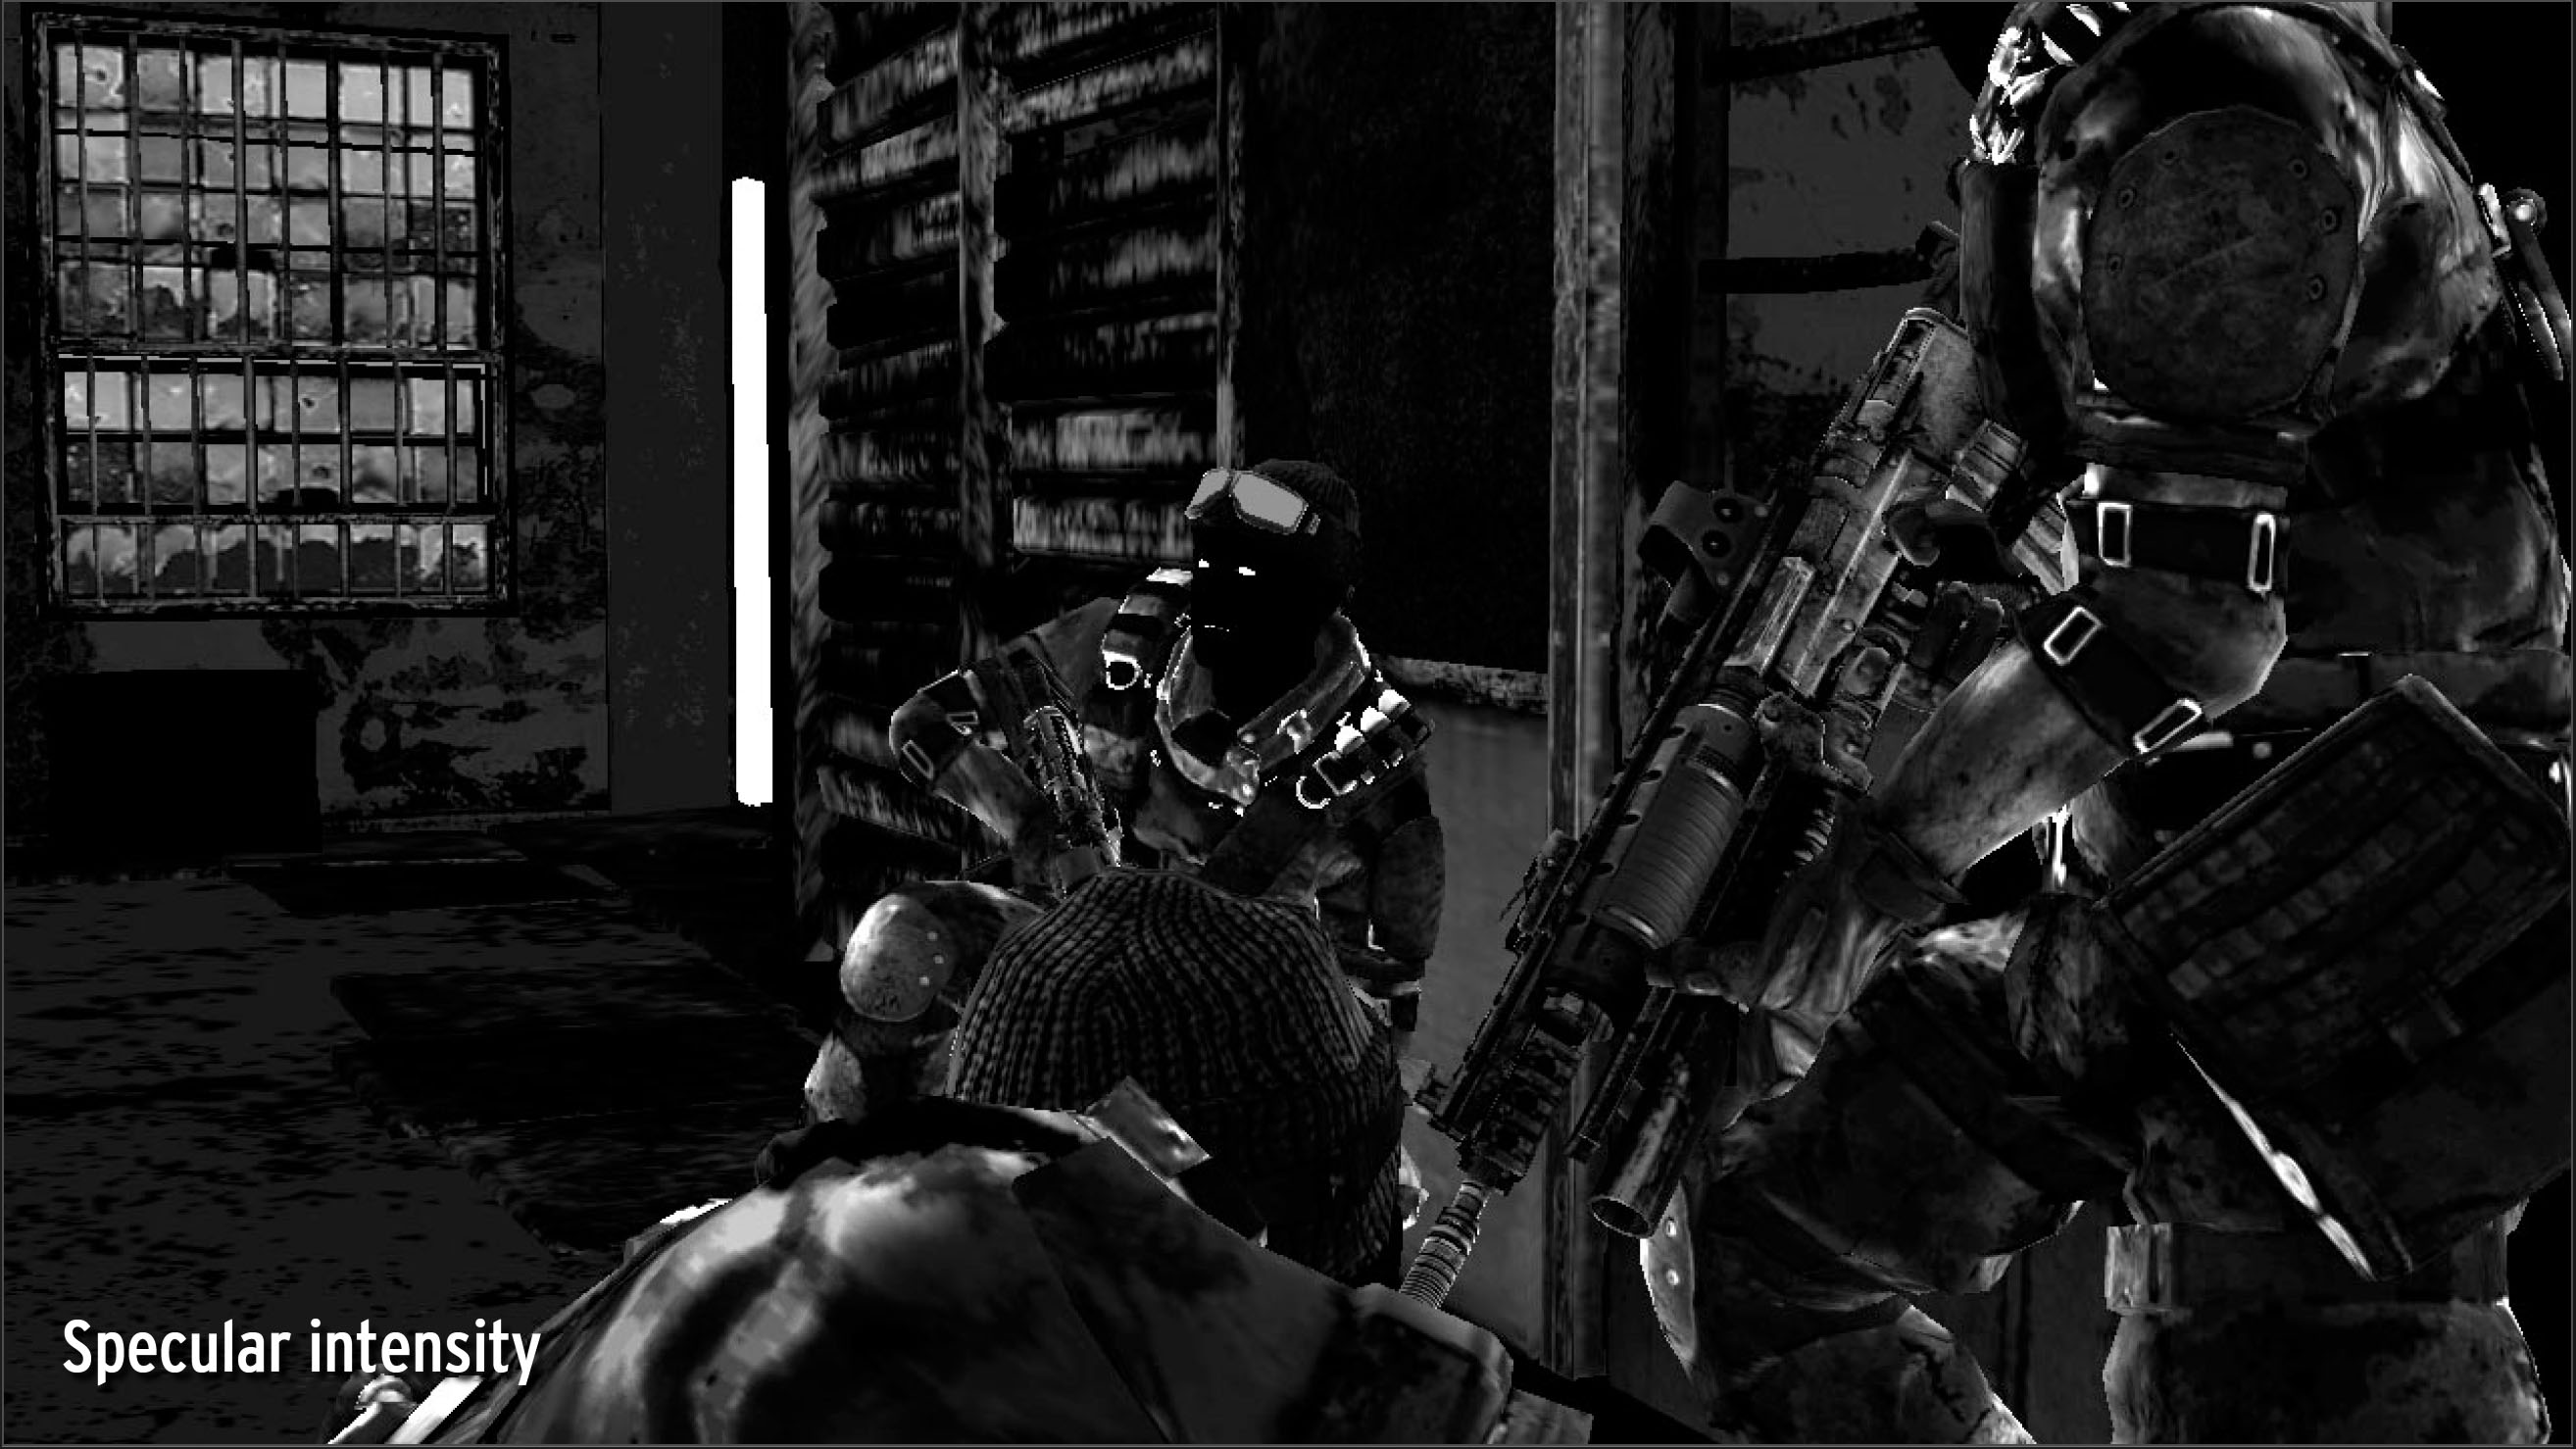
\includegraphics[width=175px]{images/graphics/killzone-2-buffer-specular.jpg}
    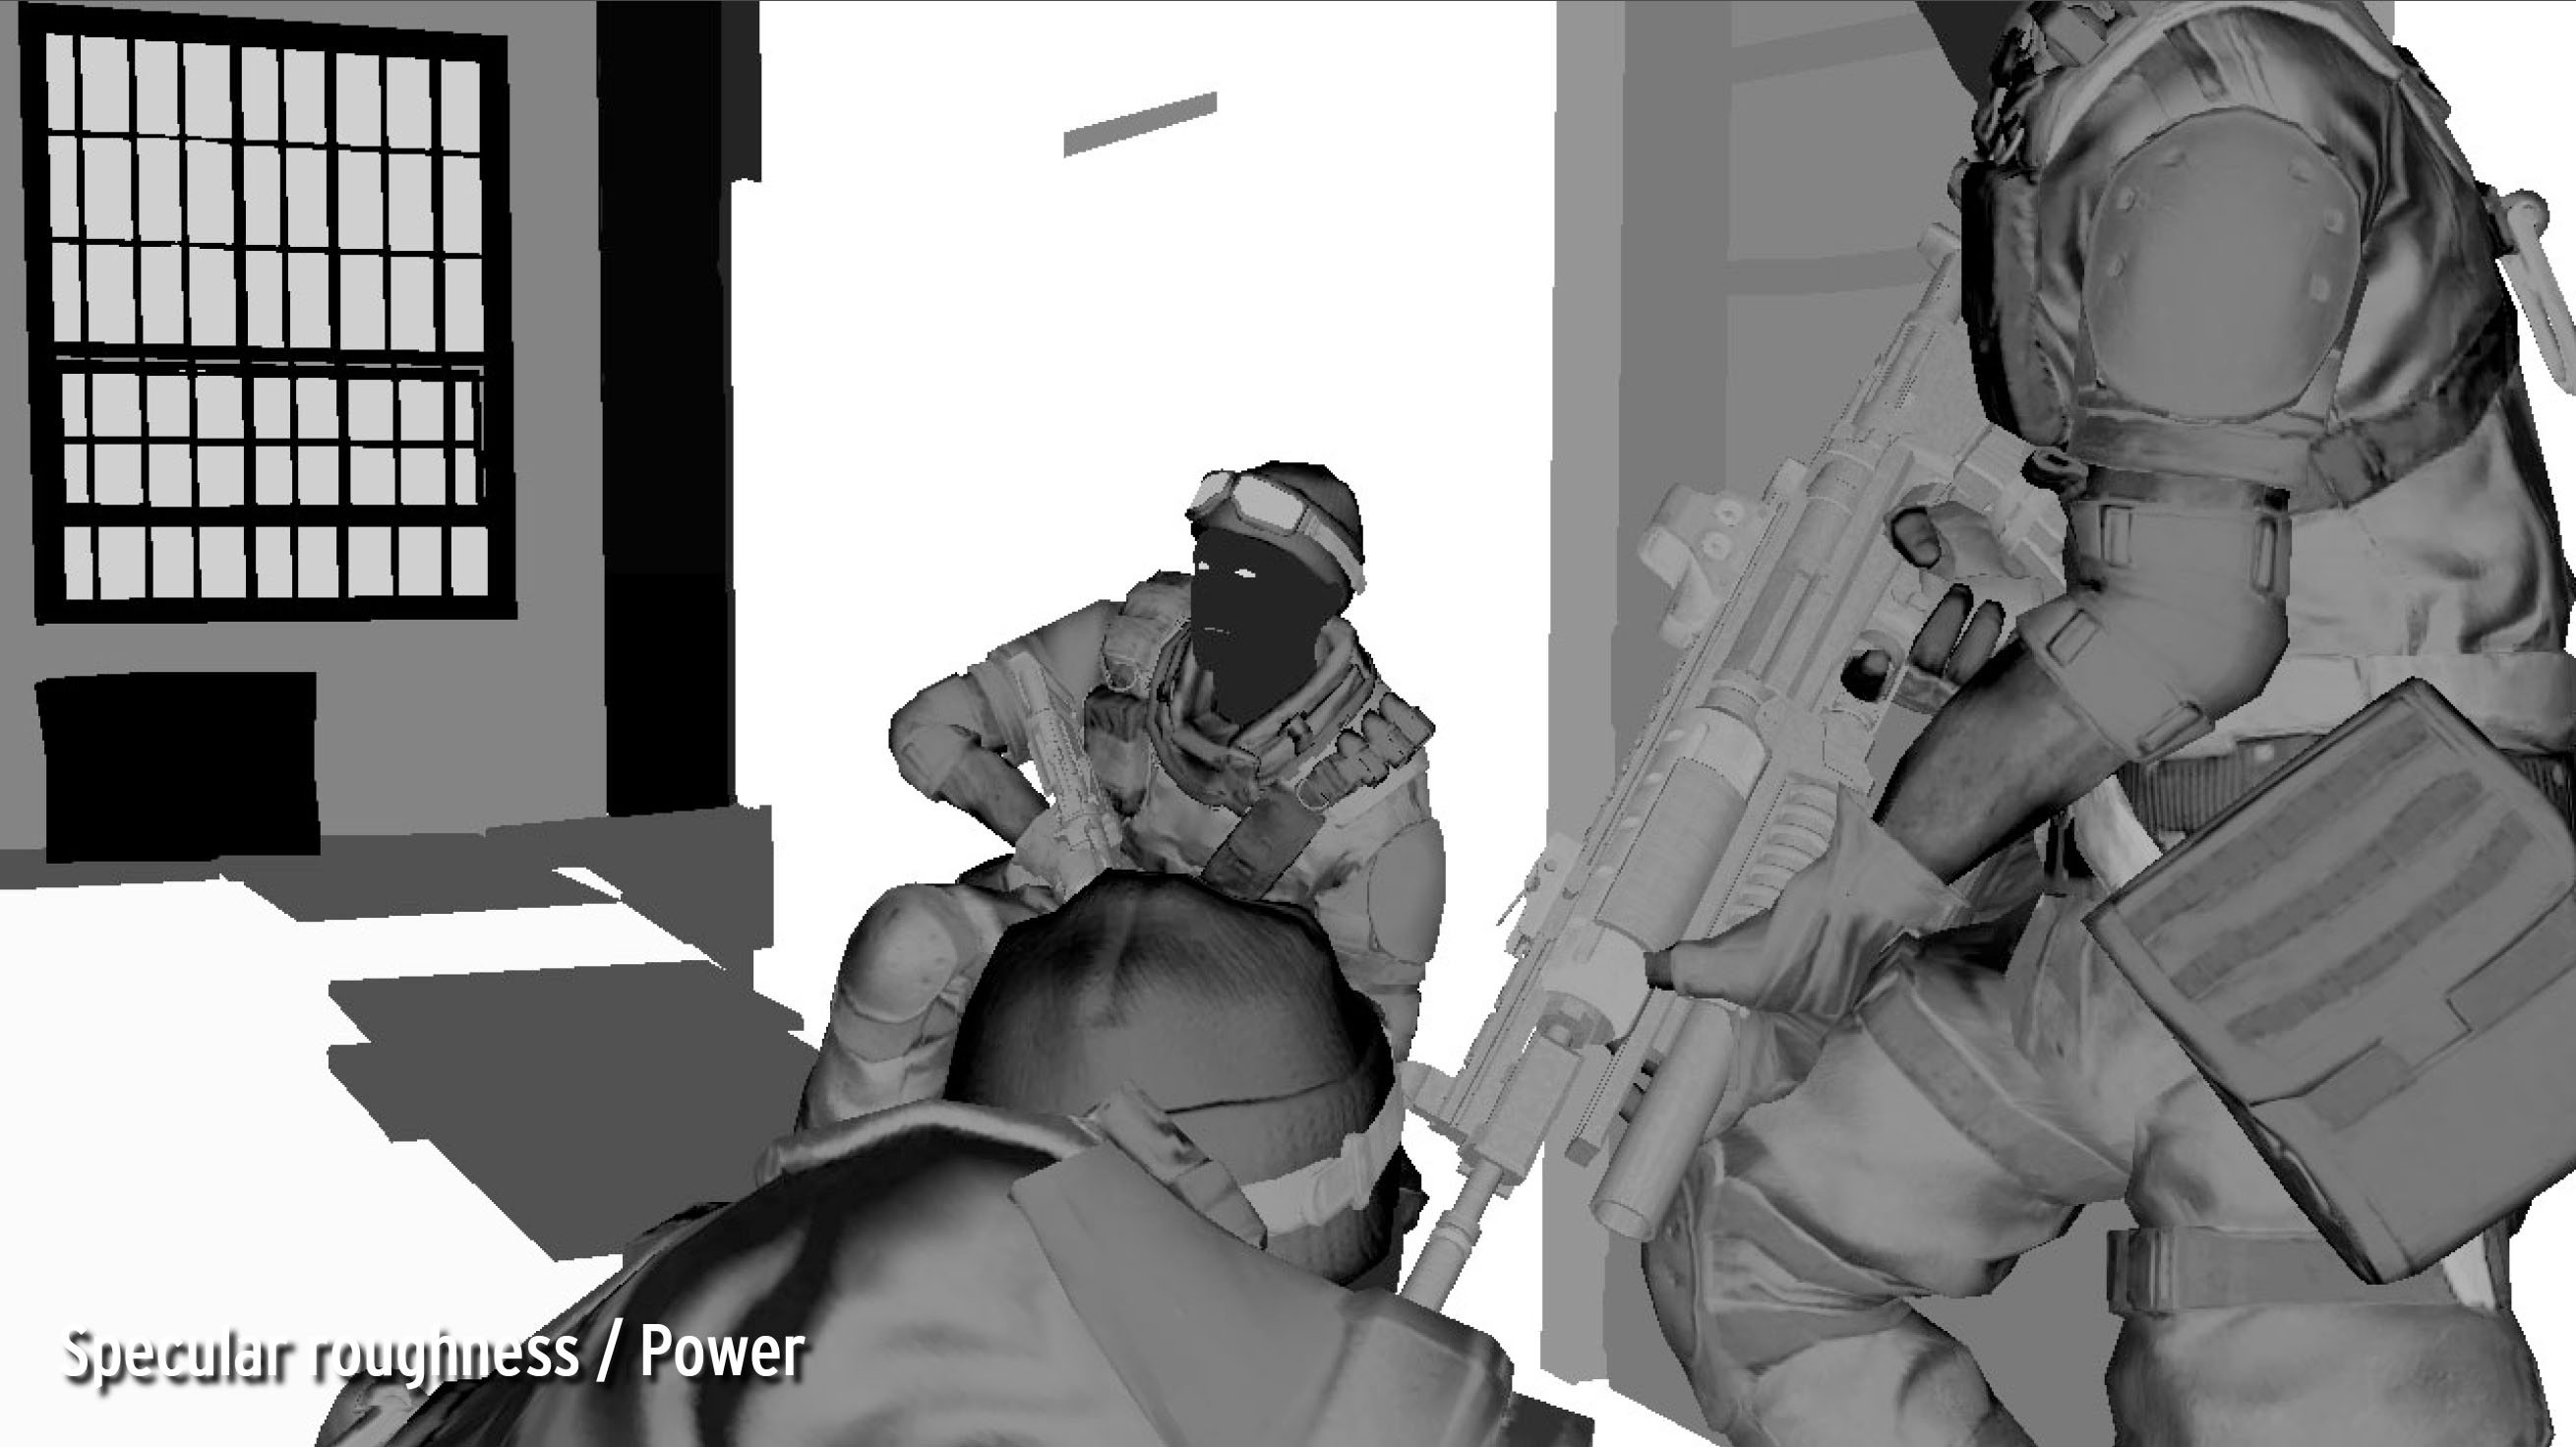
\includegraphics[width=175px]{images/graphics/killzone-2-buffer-specular-rough.jpg}
    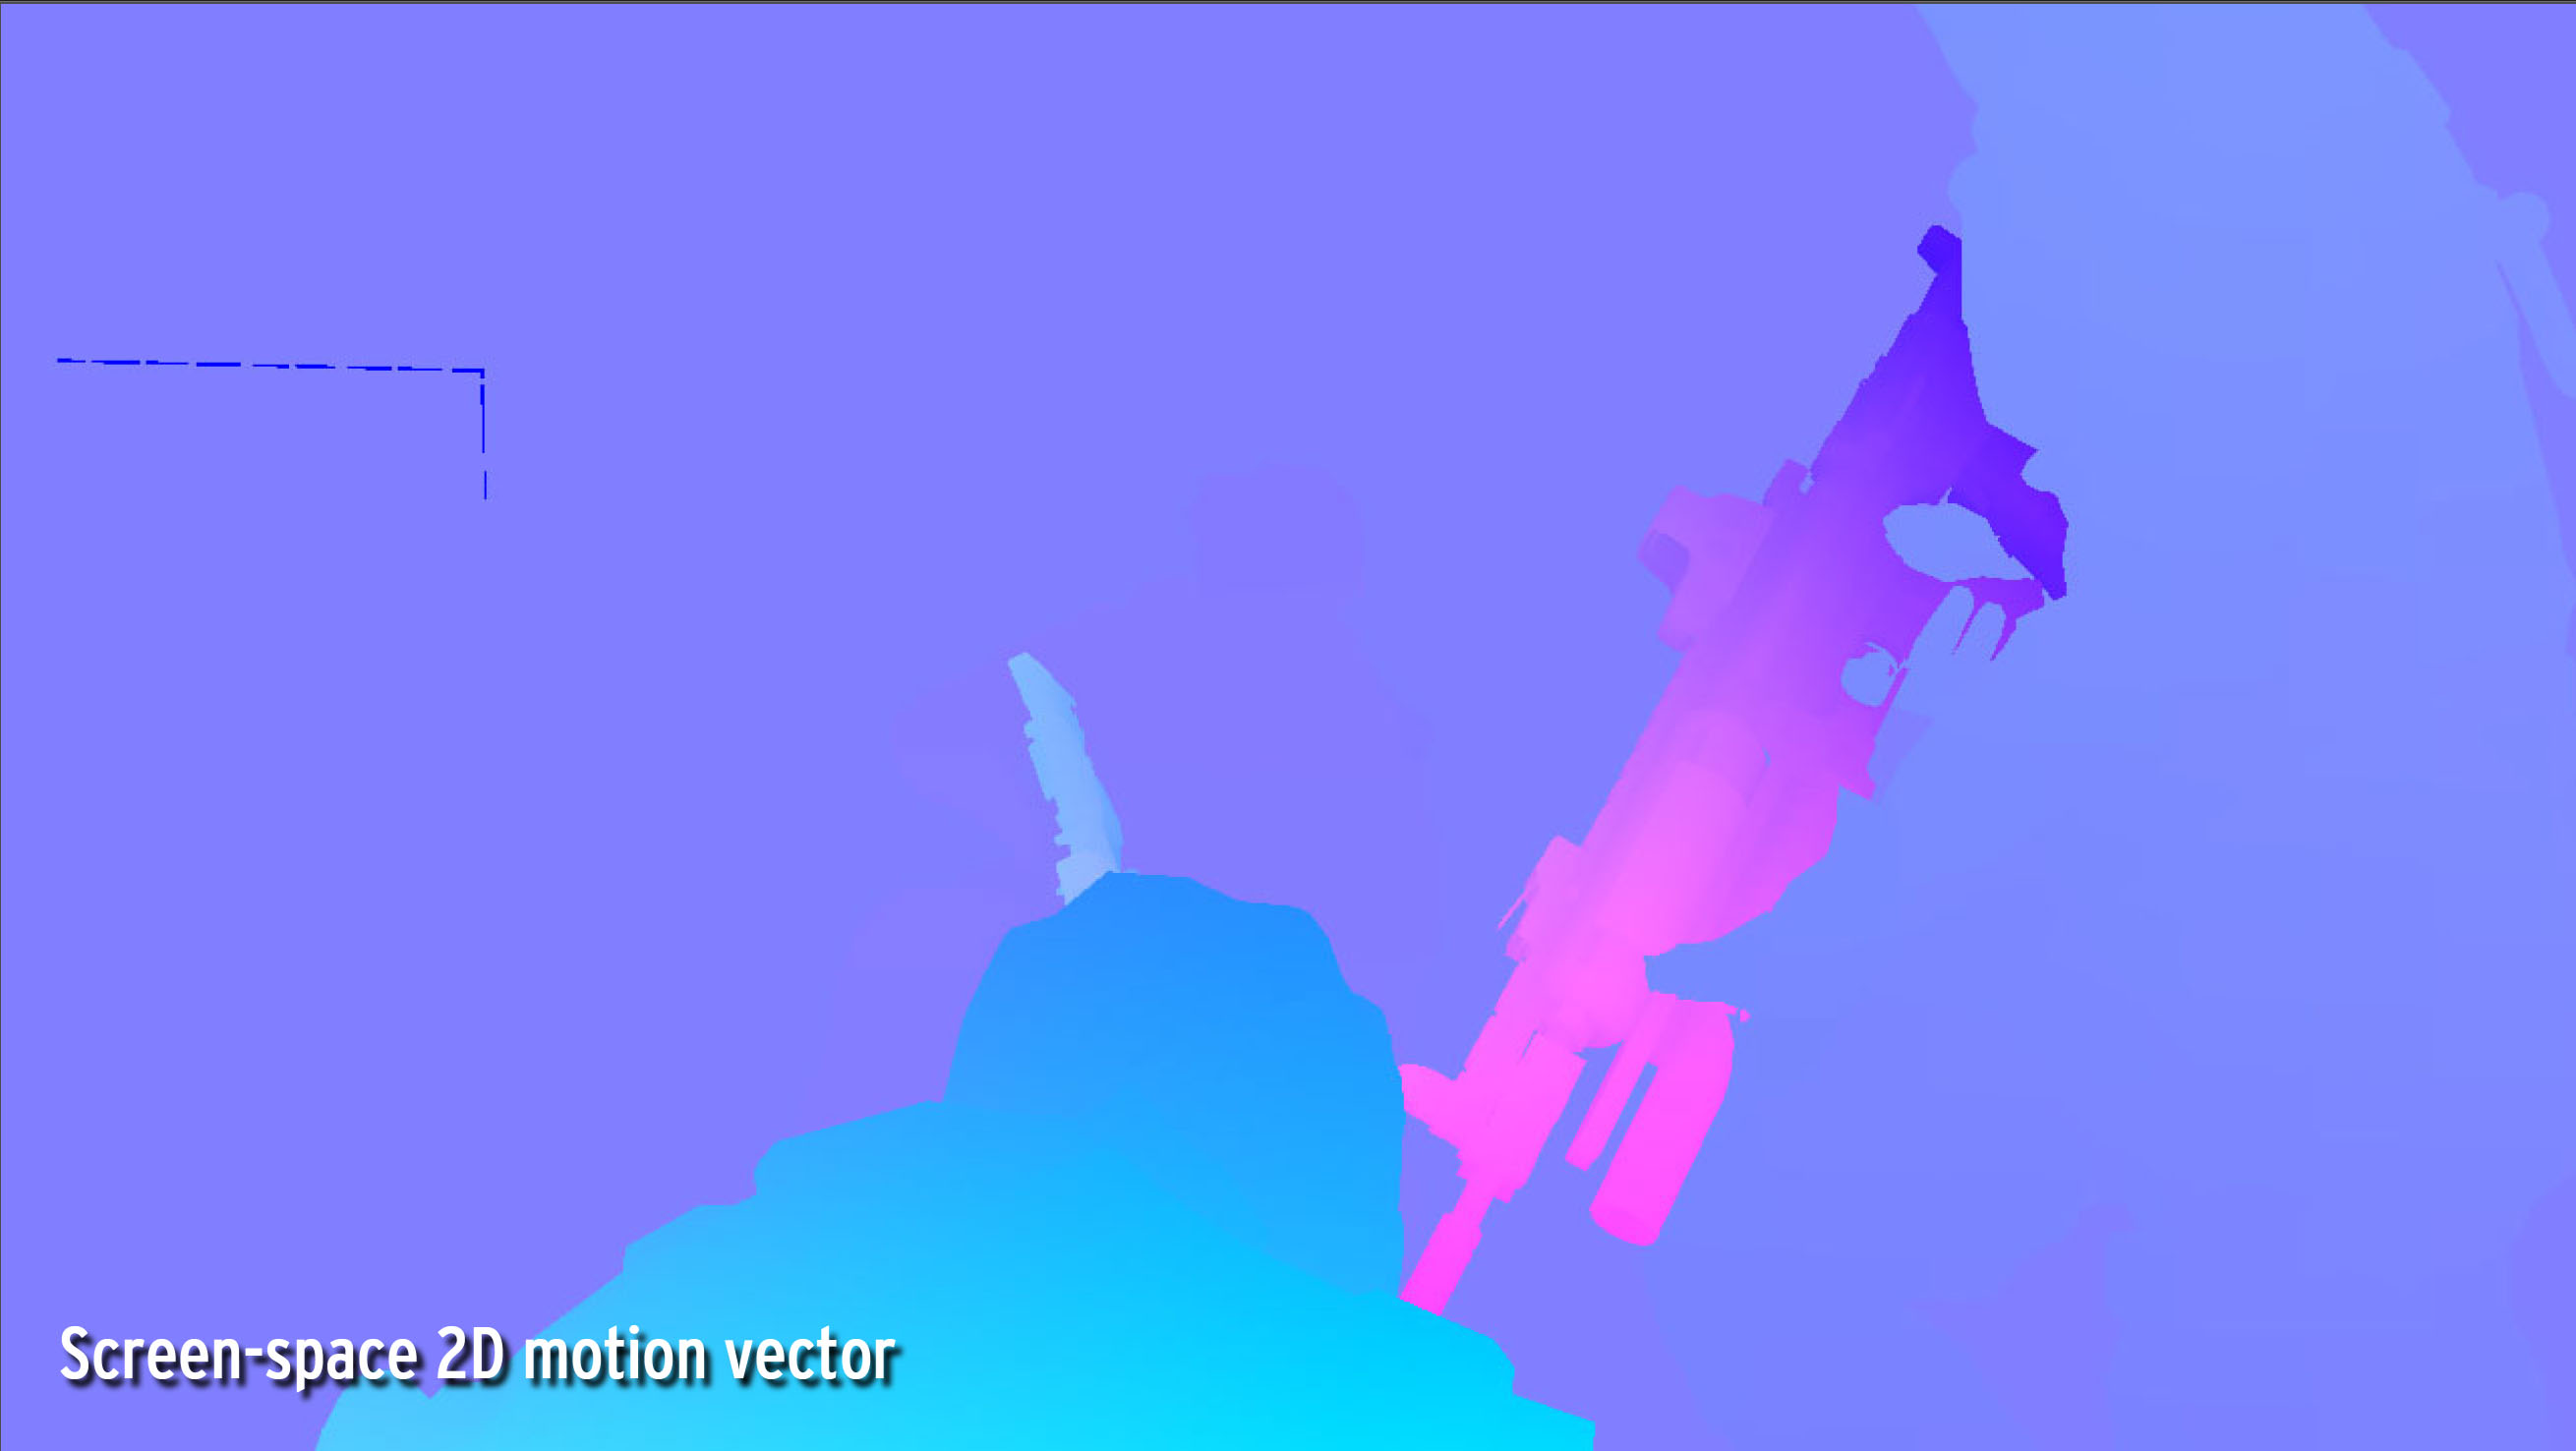
\includegraphics[width=175px]{images/graphics/killzone-2-buffer-ss-motion.jpg}
    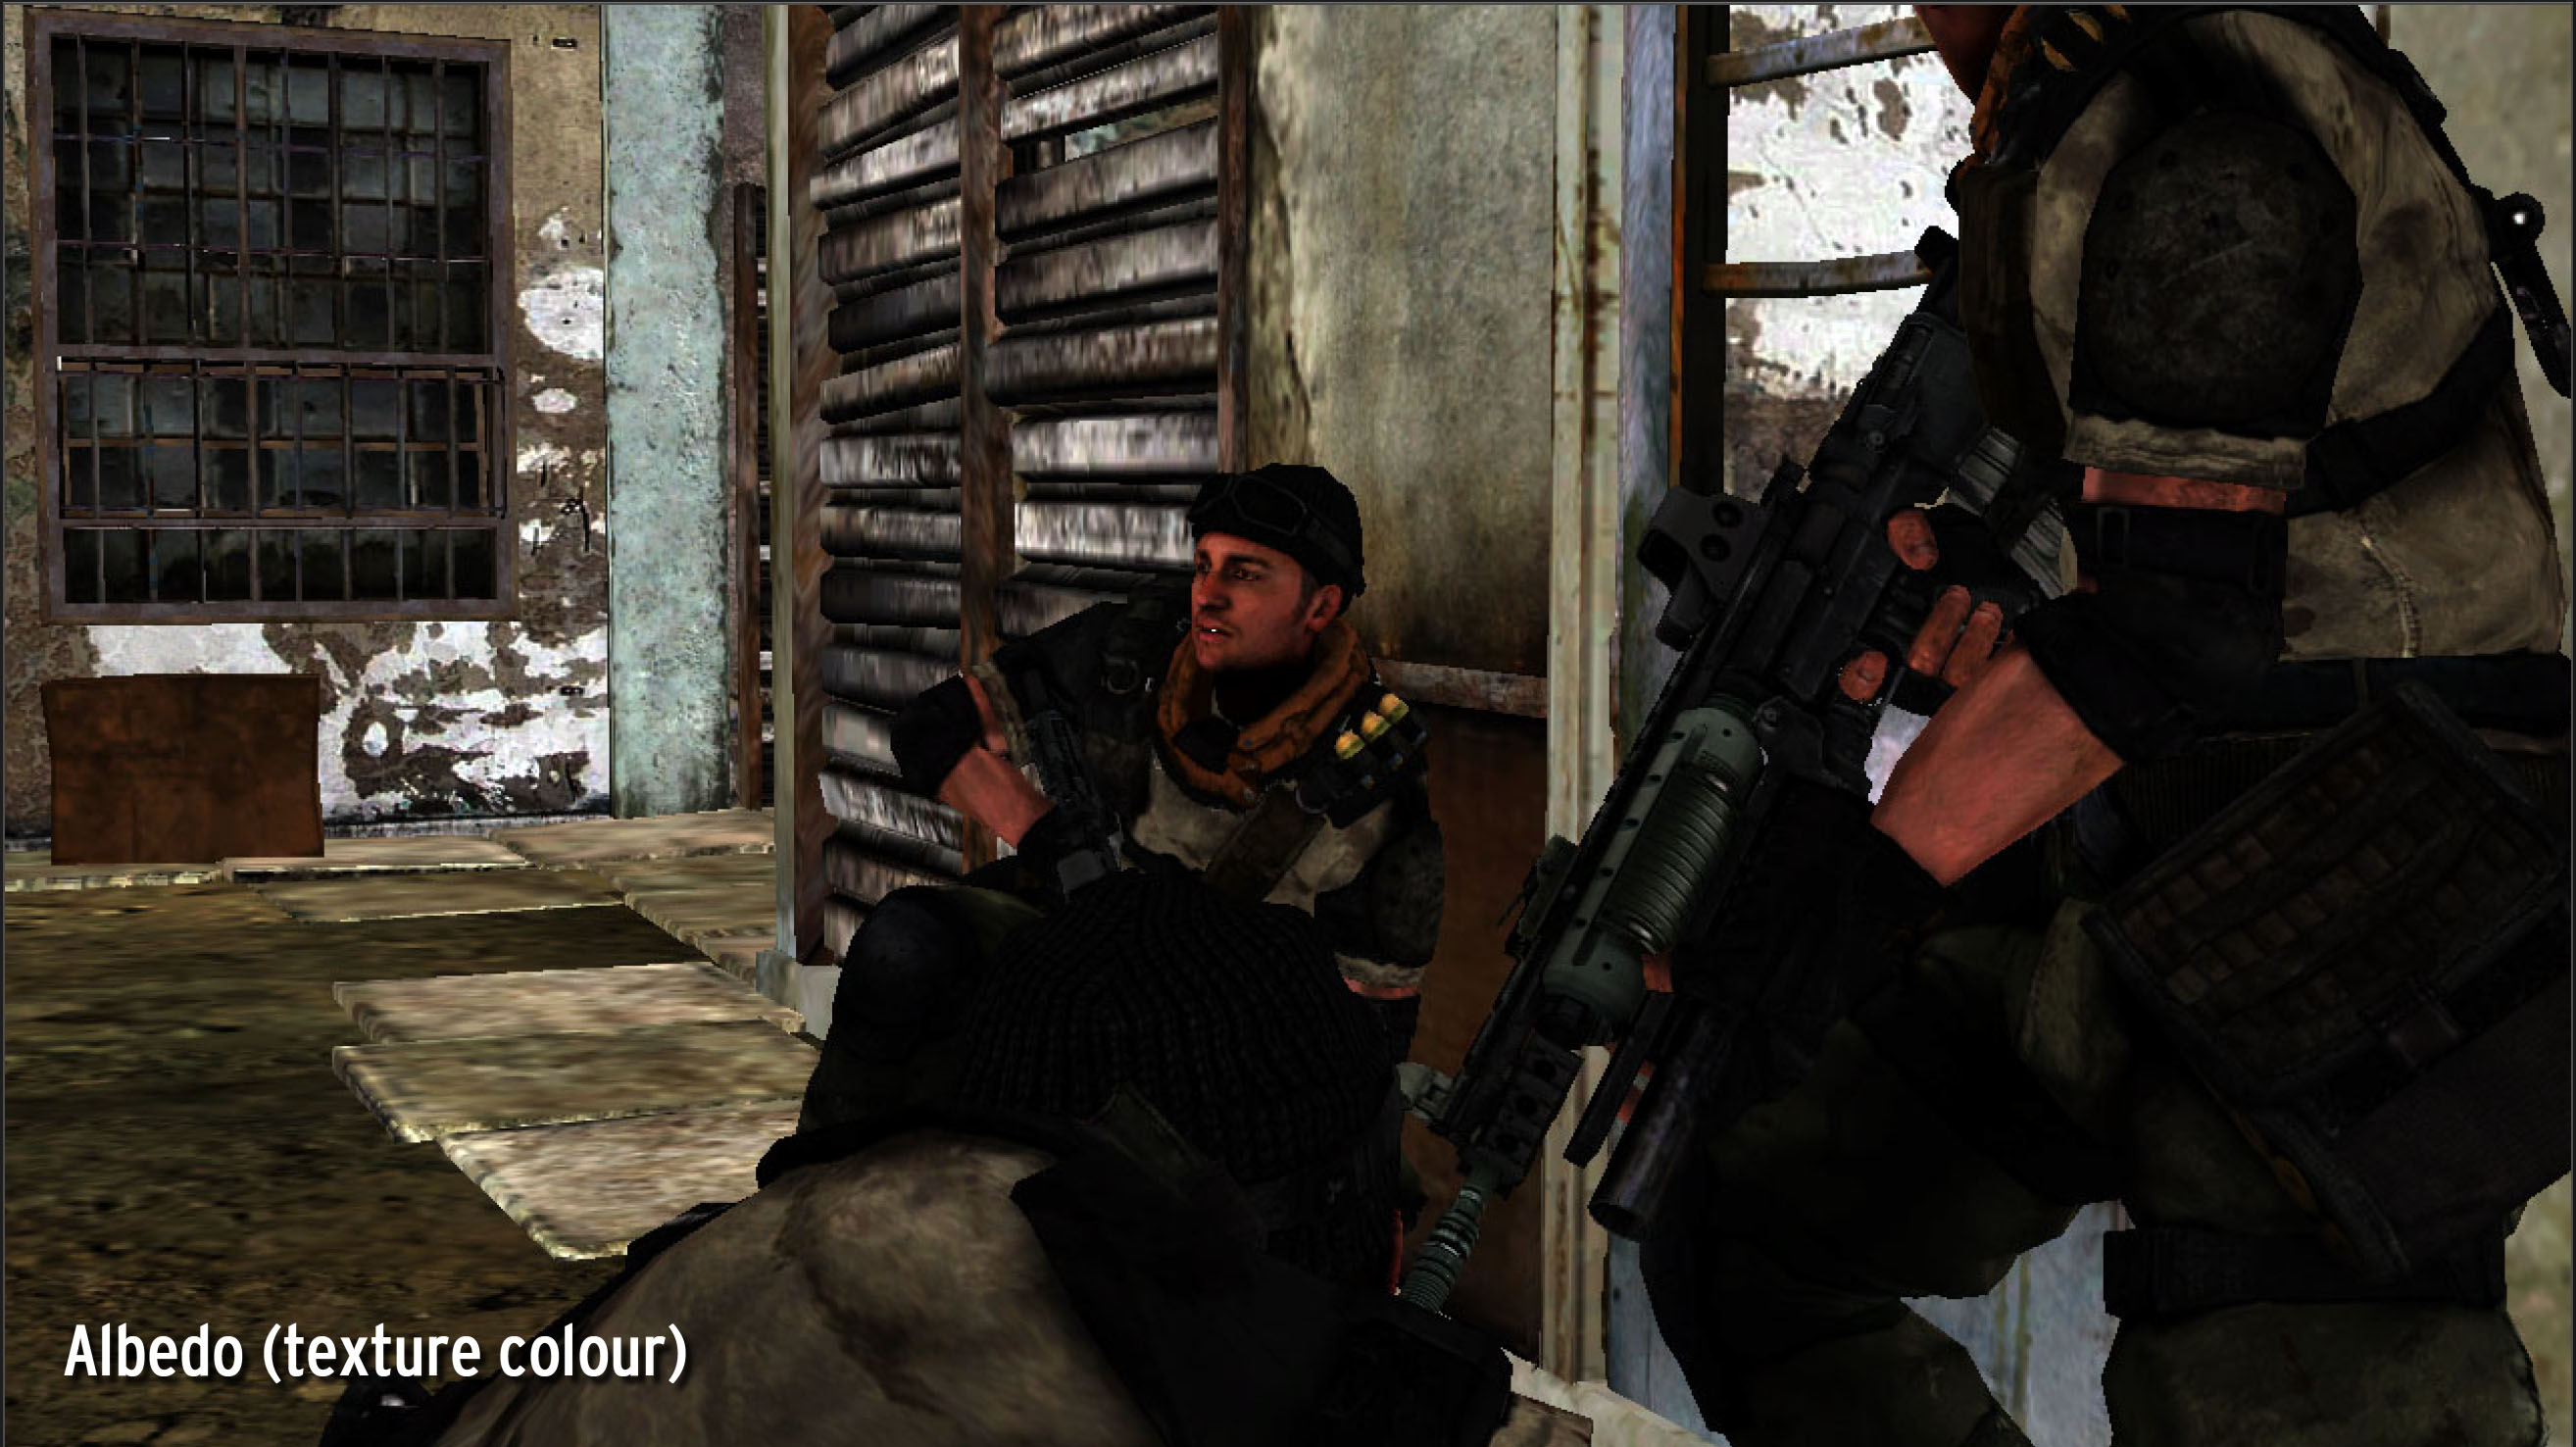
\includegraphics[width=175px]{images/graphics/killzone-2-buffer-albedo.jpg}
    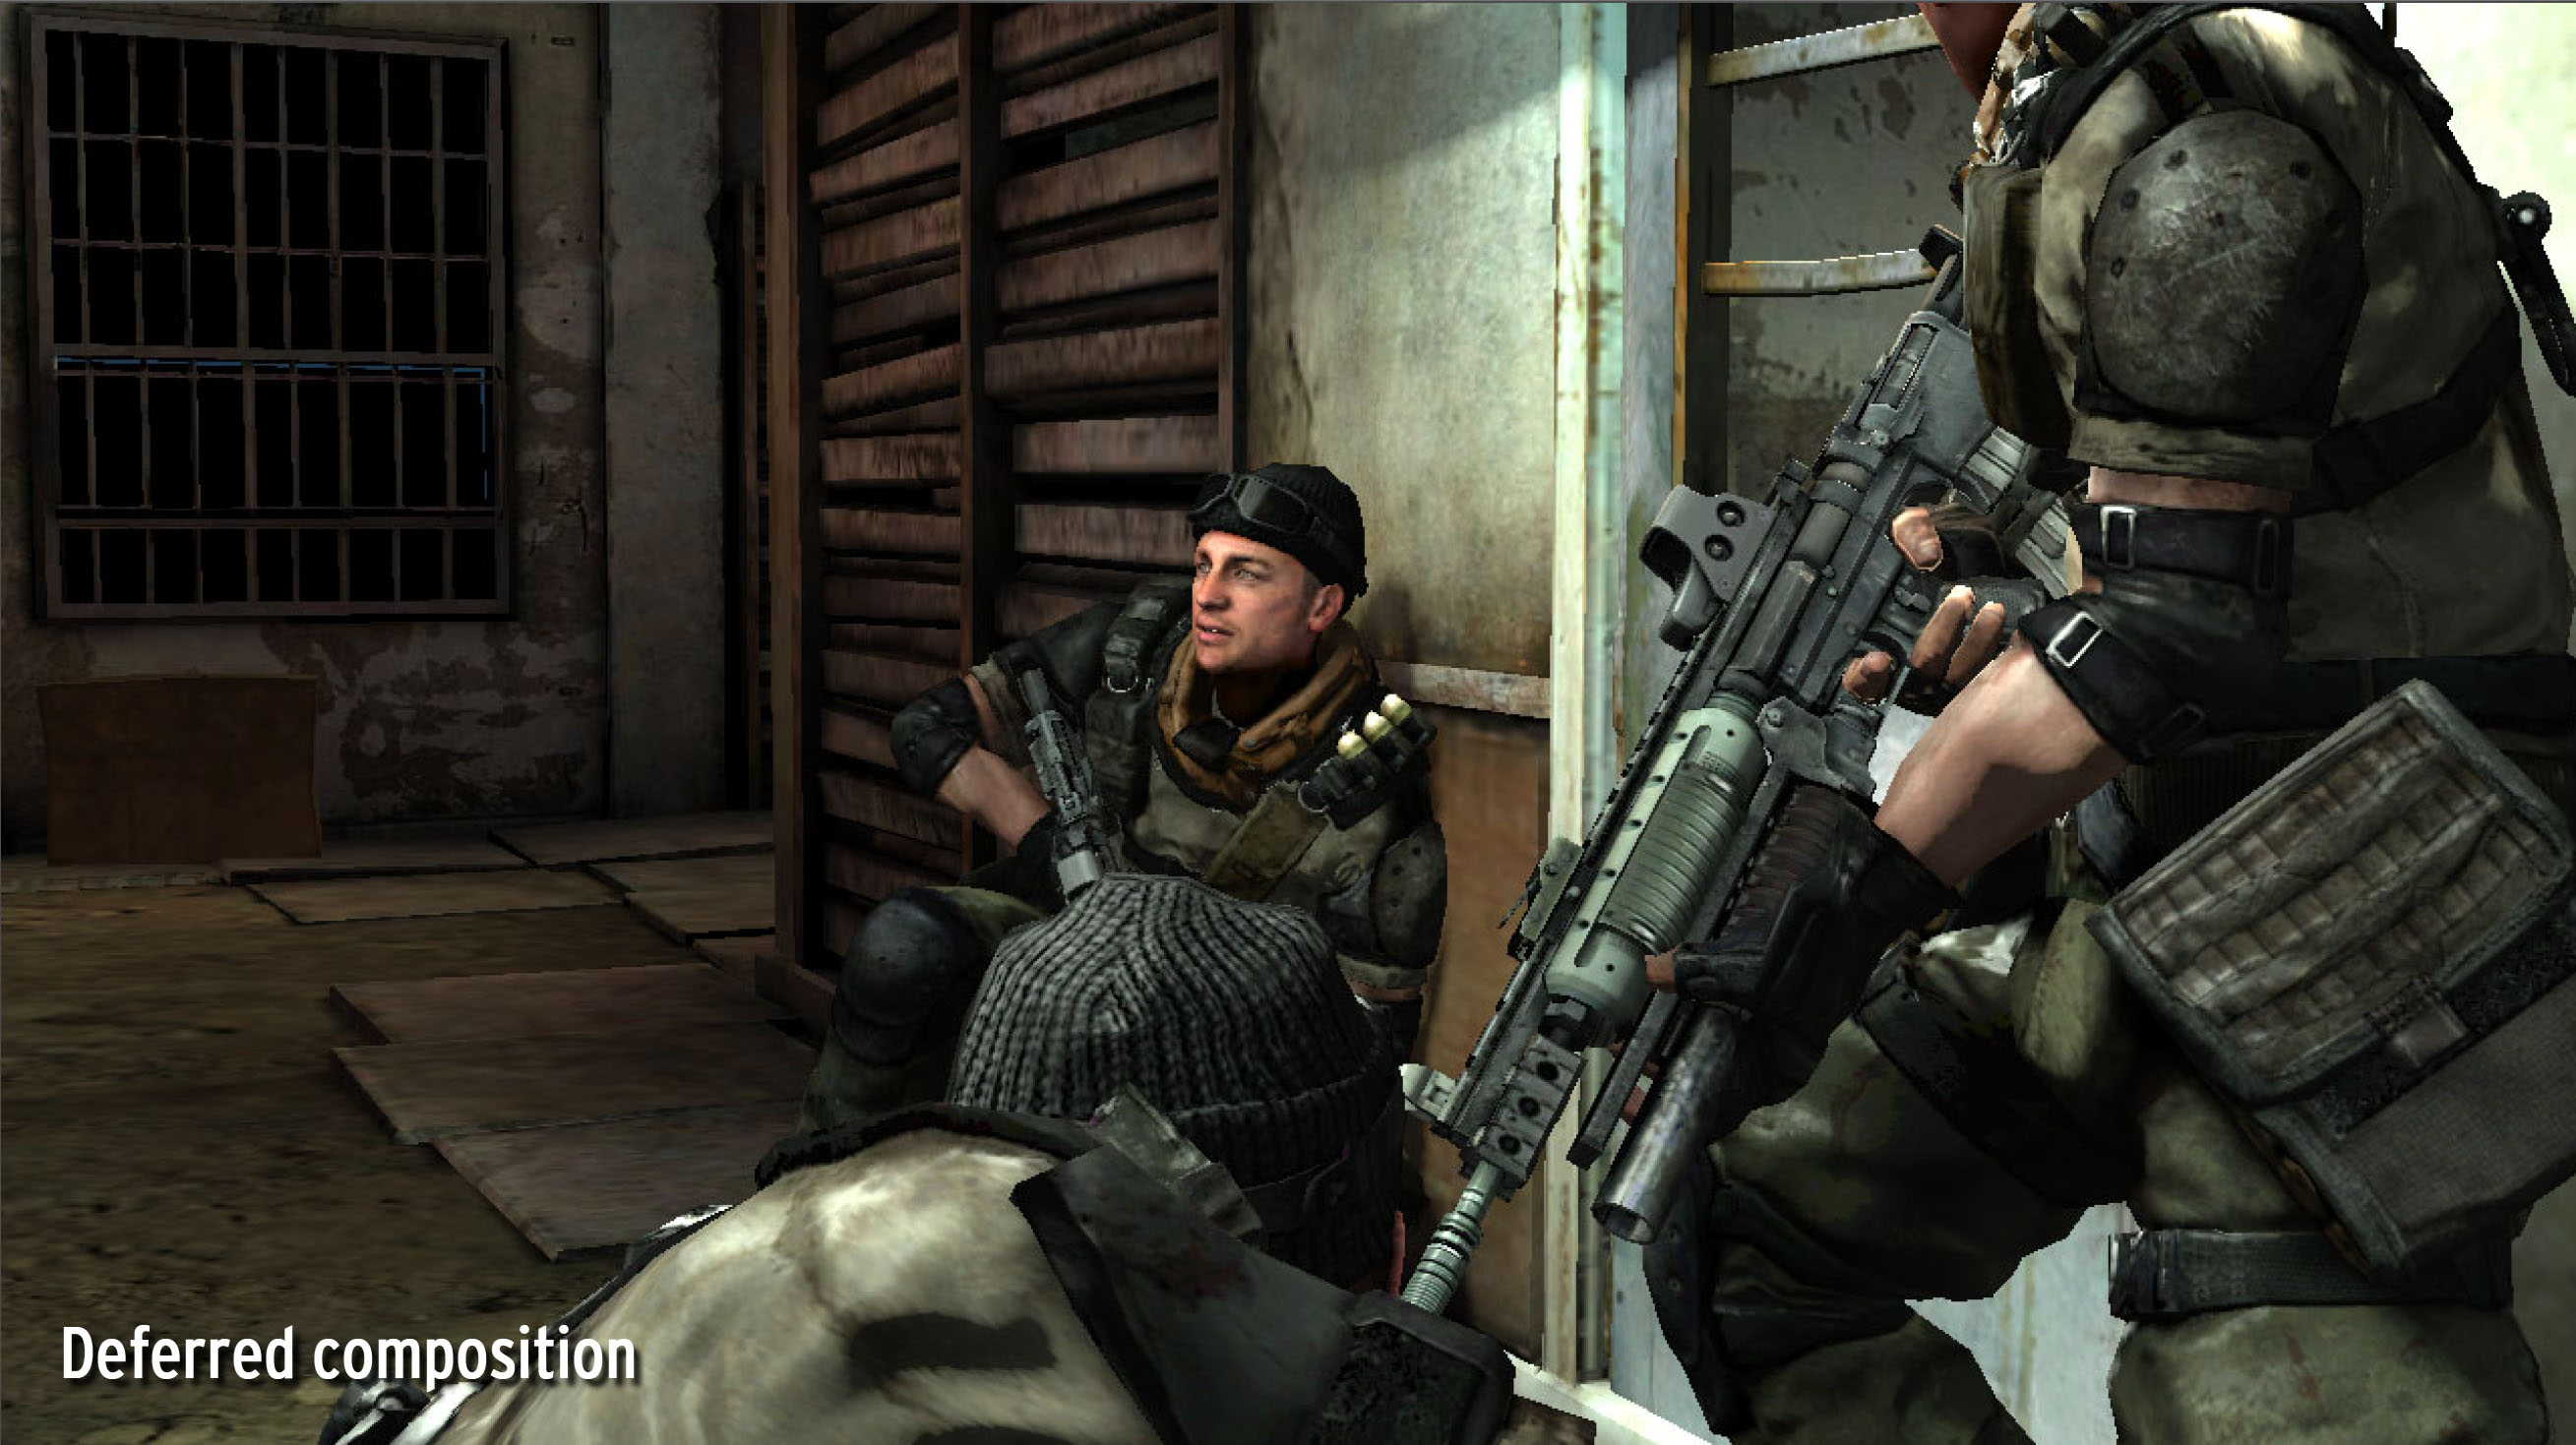
\includegraphics[width=175px]{images/graphics/killzone-2-buffer-composed-result.jpg}
    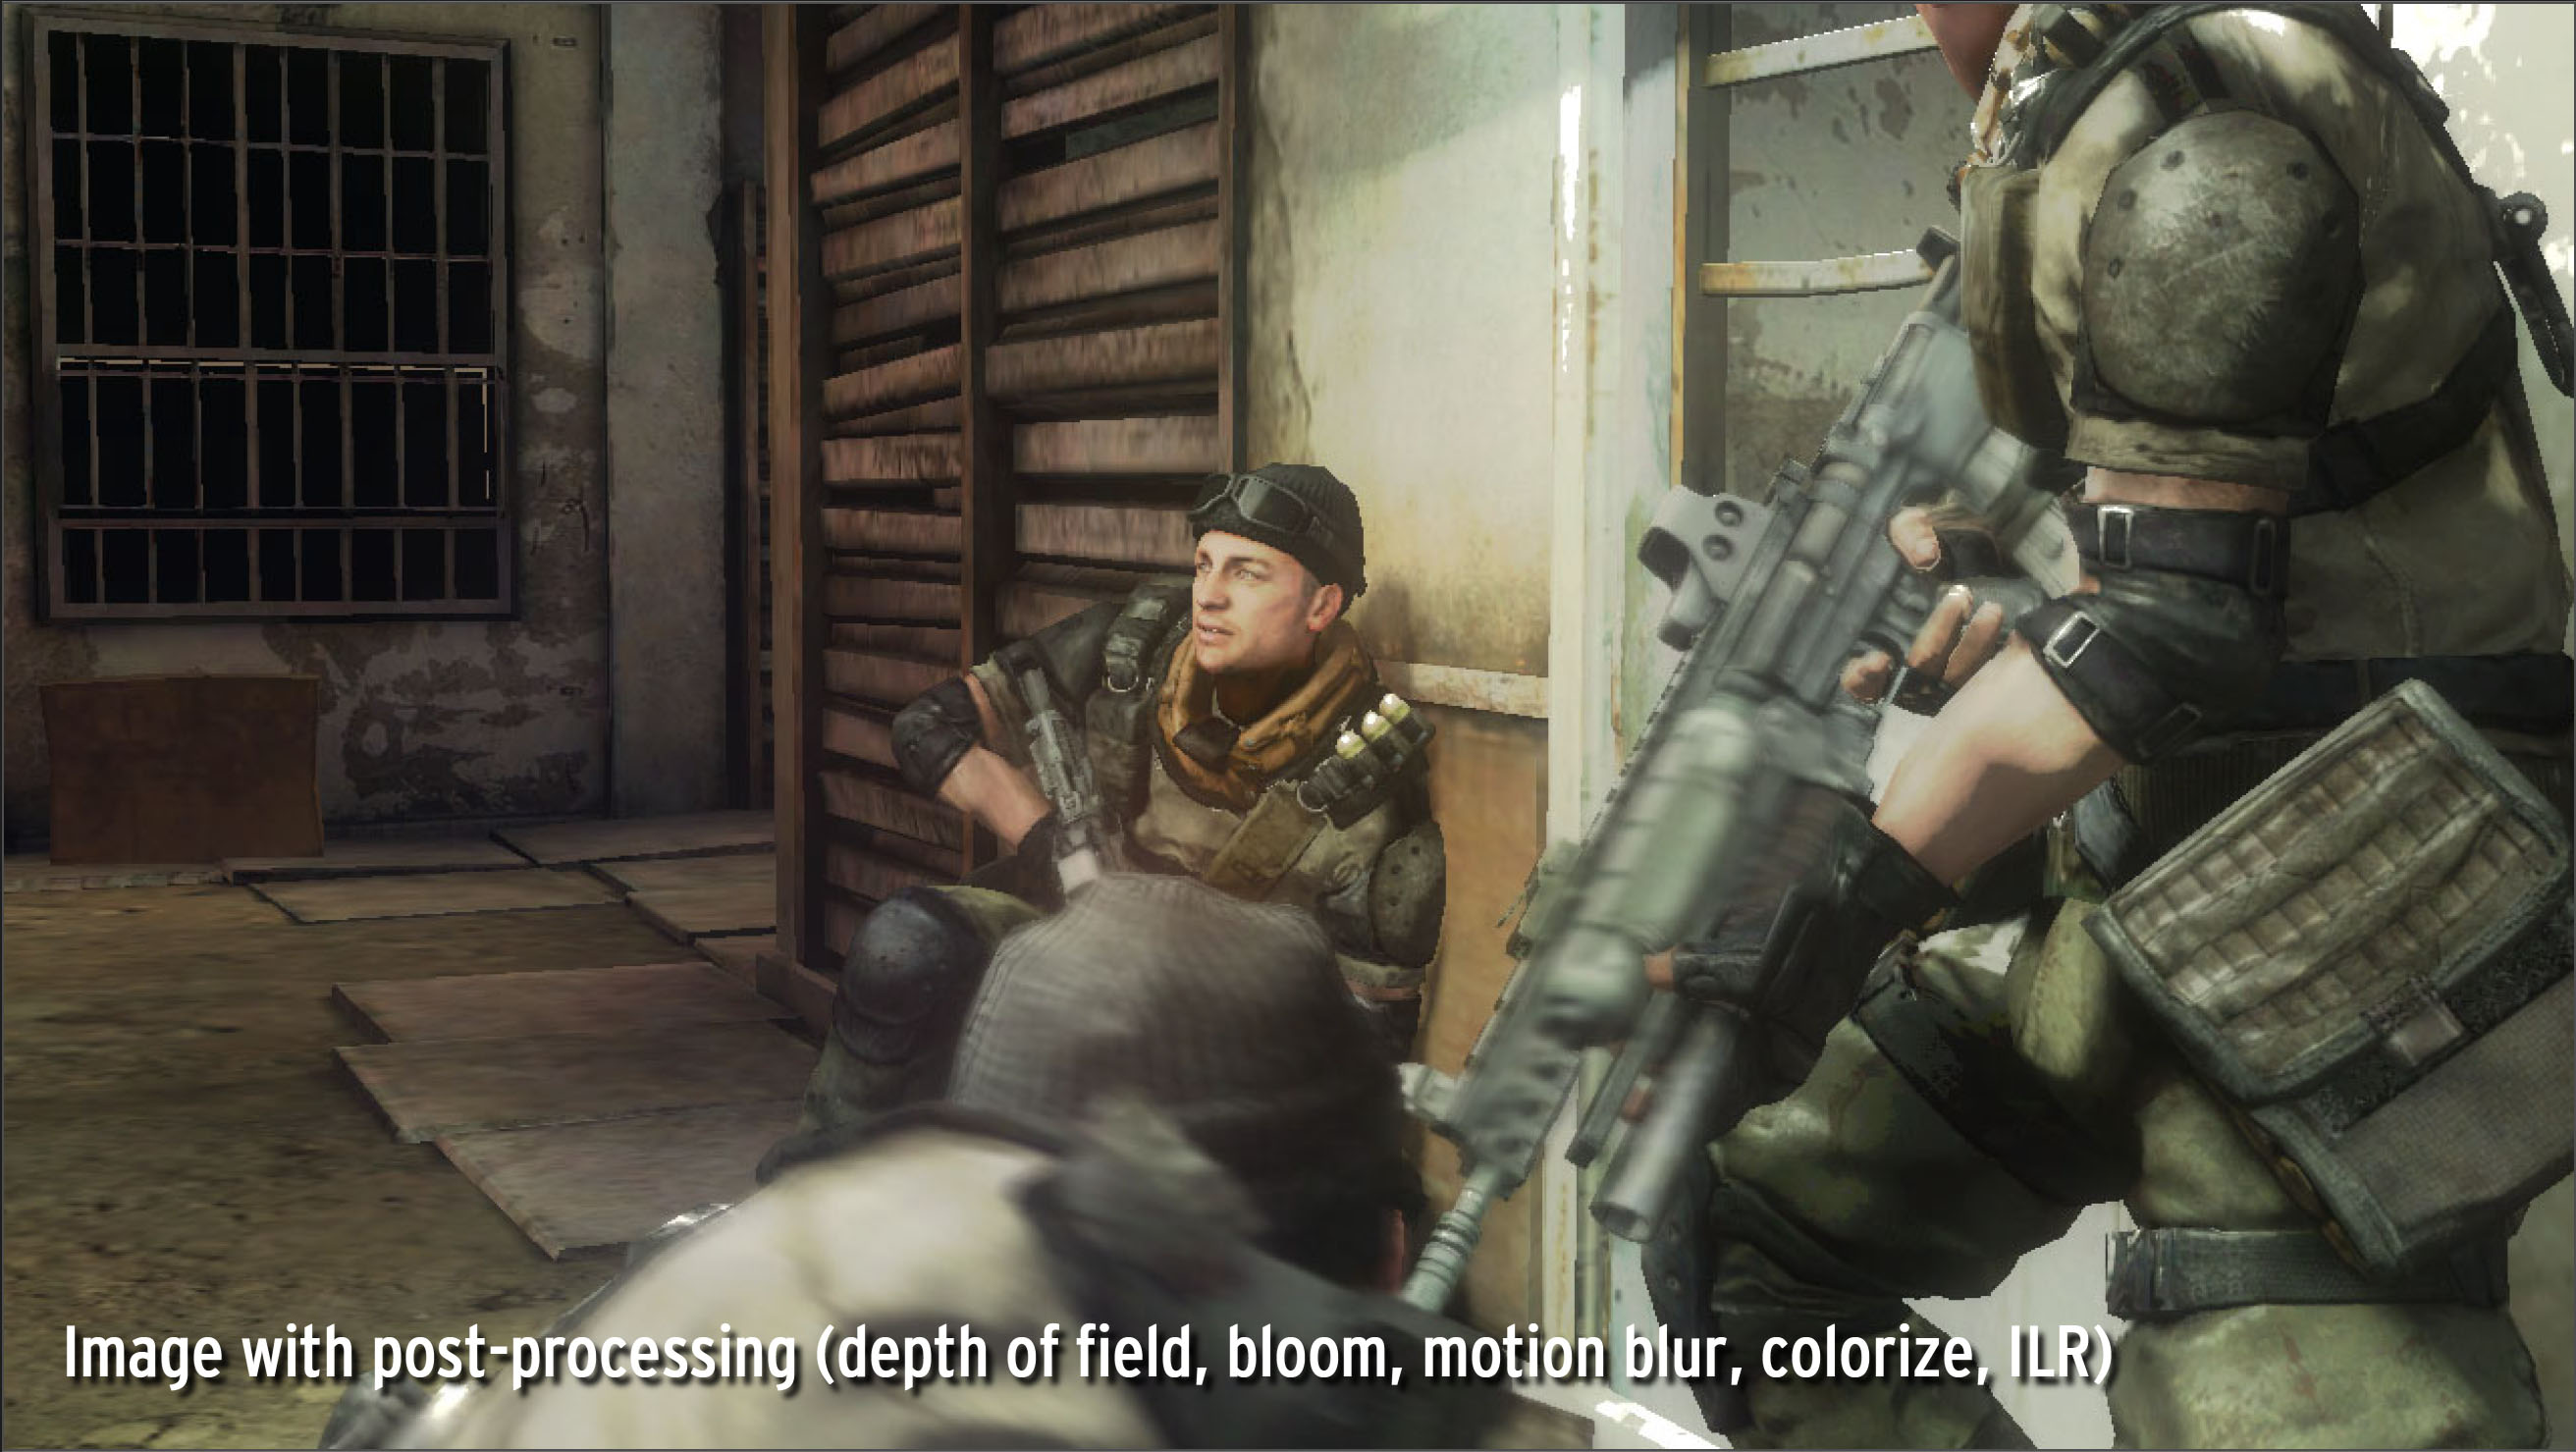
\includegraphics[width=175px]{images/graphics/killzone-2-buffer-post.jpg}
    \caption{Different buffers for \emph{Deferred Shading} in \emph{Guerilla Games'} \emph{Killzone 2} (2009) 
    \cite{Valient2007}.}
    \label{fig:deferred-shading-buffers}
\end{figure}

\noindent
As Akenine-Möller et al. point out, "the contribution of the models’ geometry has been fully decoupled from lighting 
computations" \cite{AkenineMoeller2018}. \emph{Deferred Shading} encompasses a lot more optimizations, like compression, 
light clustering, deferred texturing, and more \cite{AkenineMoeller2018}. All these techniques combined can ultimately 
result in a more efficient shading model for specific use cases, for instance, when using a lot of lights in combination 
with high density geometry.\\

\noindent
The basic idea of \emph{Deferred Shading} influenced the next couple of years of real-time graphics technology and is 
still used today for state-of-the-art game development. Dispatching work for the \ac{GPU} and optimizing memory and 
data layouts for most efficient computation has contributed to \ac{GPUDR} to become one of the latest trends in real-time 
rendering.

\subsection*{GPU Driven Rendering}

\begin{figure}[h]
    \centering
    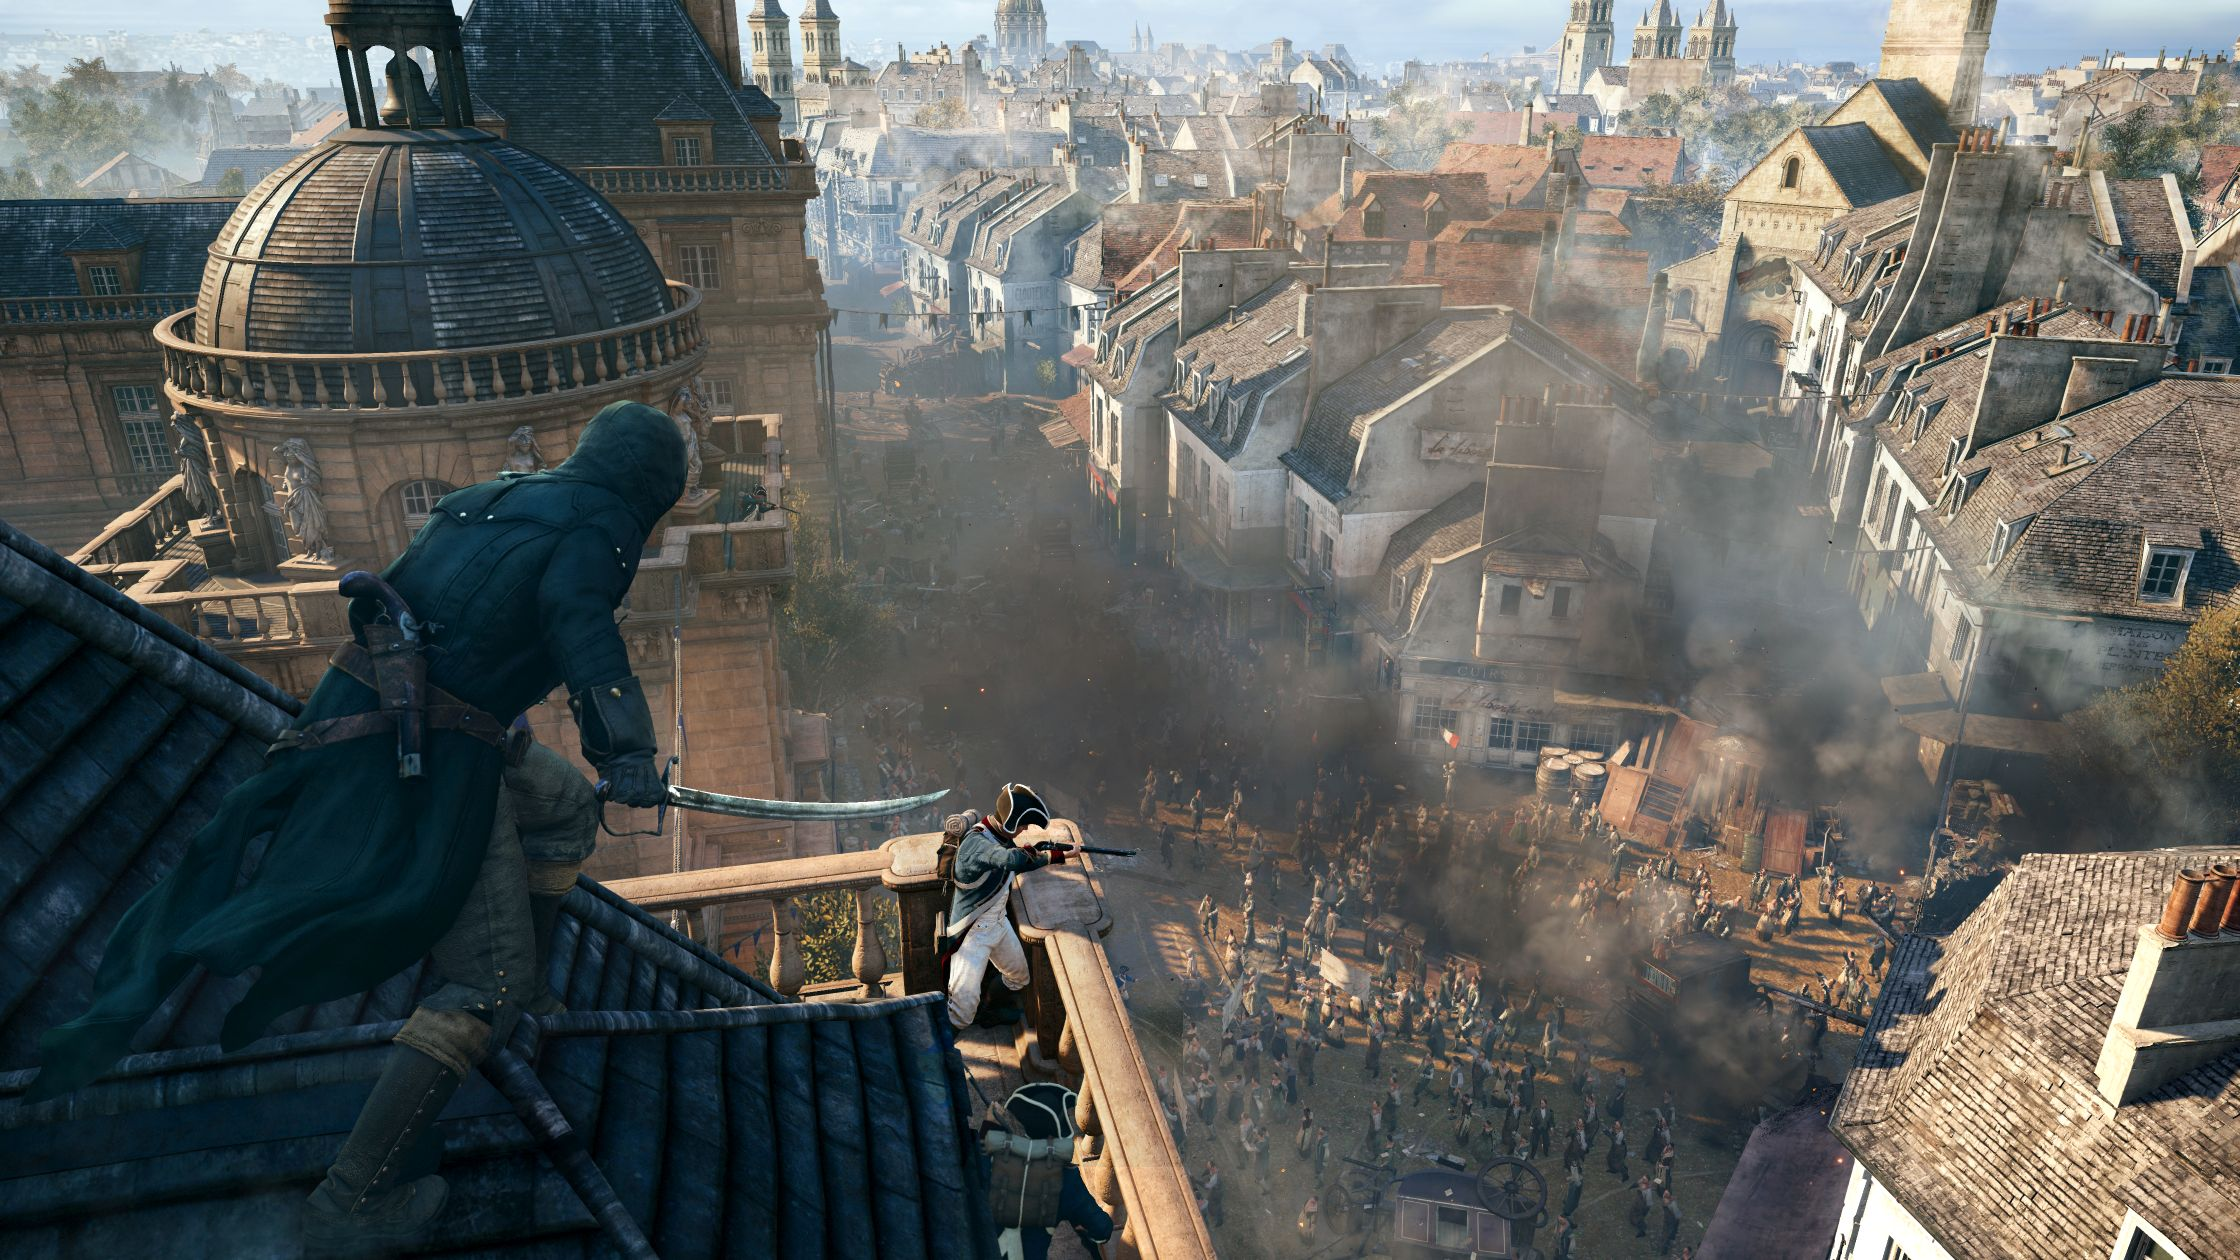
\includegraphics[width=300px]{images/graphics/assassins-creed-unity-gameplay.jpg}
    \caption{A screenshot of the game \emph{Assassin's Creed Unity} (\emph{Ubisoft} \cite{Ubisoft2014}, 2014) 
    showcasing the high density of geometry and far draw distances \cite{Burke2014}.}
    \label{fig:assassins-creed-unity-gameplay}
\end{figure}

\noindent [@TODO: Sources]
Over a decade after the first \ac{GPU} was introduced, hardware acceleration was the de facto standard in 
computer graphics, and the rendering pipeline got more and more loaded with features, innovations, and data. 
This led to a new bottleneck: the memory bandwith between the \ac{CPU} and \ac{GPU}. Soon, a new trend was 
developed: \emph{\ac{GPUDR}}. The goal of \ac{GPUDR} is to minimize bandwidth between \ac{CPU} and \ac{GPU}. 
An ideal \ac{GPU} driven application would only update the camera-related data (view and projection matrices) 
within a frame. All computations would be issued by the \ac{GPU} itself, potentially leading to new computations 
issued directly on the \ac{GPU}. This way, no synchronization between \ac{CPU} and \ac{GPU} is necessary, and the 
complete scene can be rendered in a single \ac{CPU} draw call. However, for this to work, data has to be laid out 
in a \ac{GPU}-friendly way, representing data relationships in a way that can be processed by shaders efficiently. \\

\noindent
This trend gained attention with the rise of the \ac{GPGPU} and the better support for the more generalized 
\emph{compute shaders}. The definition for when applications are \ac{GPU} driven or not is blurred, but one 
of the earlier games to make heavy use of \ac{GPUDR} is \emph{Assassin's Creed Unity} (\emph{Ubisoft} 
\cite{Ubisoft2014}, 2014), shown in Figure \ref{fig:assassins-creed-unity-gameplay}. In 2015, Aaltonen et al. 
\cite{Aaltonen2015} presented approaches for \ac{GPUDR}, which included \emph{Occlusion Culling},
\emph{Deferred Texturing}, and the clustering of geometry. The proposed technology allowed for a densely populated, 
dynamic, open world. Some of the technology used would only be seen in other games almost a decade later, when 
geometric computation was supported by specific hardware adaptations. Especially large, open games can profit from 
optimizations like storing scene data directly on the \ac{GPU}. In modern real-time computer graphics, the 
pre-computation by the \ac{CPU} and the data transfer to the \ac{GPU} are replaced by data generation on the 
\ac{GPU} itself.

\subsection*{Mesh Shading Pipeline} \label{subsec-mesh-shading-pipeline}


\begin{figure}[h]
    \centering
    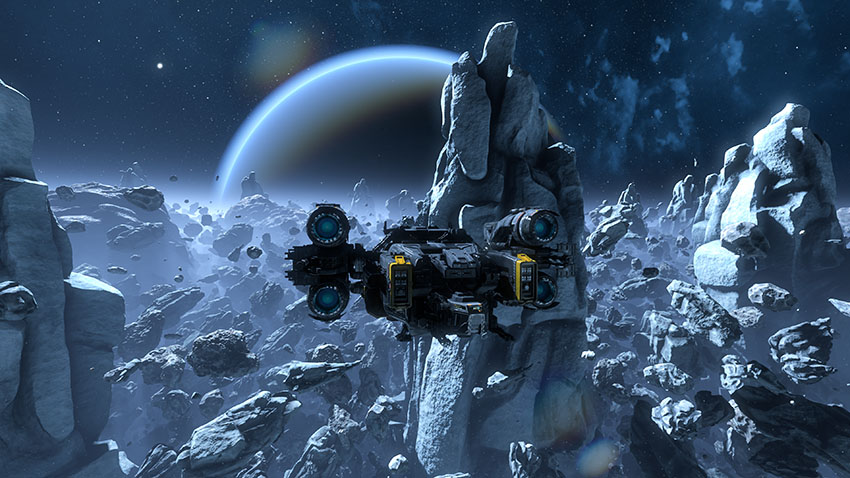
\includegraphics[width=300px]{images/graphics/mesh-shading-asteroids-demo.jpg}
    \caption{The offical \emph{Mesh Shading Pipeline} \emph{Asteroids} demo, featuring the new \emph{Mesh Shading Pipeline} (2018)
    and a high geometric density \cite{Kraemer2018}.}
    \label{fig:mesh-shading-asteroids-demo}
\end{figure}

\noindent
More elaborate algorithms for data computation on the \ac{GPU} led to a further increase in geometrical density.
This is why \emph{NVIDIA} introduced the new \emph{Mesh Shading Pipeline} in 2018 for \emph{NVIDIA Turing} \ac{GPU}s.
This pipeline improves the "old" vertex shader and features a more flexible way of computing and drawing geometry. 
It builds upon some of the innovations presented by Aaltonen et al.  \cite{Aaltonen2015} in 2015. Figure 
\ref{fig:mesh-shading-asteroids-demo} shows one frame of the initial demo provided by \emph{NVIDIA}. Mesh Shading 
allows developers to output geometrical primitives in any way they like and breaks down geometry into small clusters.
Each cluster can be computed individually by using the compute shaders. This way, geometry can be manipulated more 
precisely than before, and the processing of the primitives additionally benefits from the highly efficient compute 
architecture, providing groupshared memory, fewer limitations, and a more flexible way of operating on geometry.
The pipeline is discussed in more detail in Chapter \ref{sec-mesh-shading} and is a central part of modern games 
such as \emph{Remedy's} Alan Wake 2 (\emph{Remedy Entertainment} \cite{AlanWake22023}, 2023) or even 
\emph{Epic Games'} \emph{Unreal Engine 5} \cite{Karis2021}. 


\section{Motivation} \label{sec-motivation}

The latest innovations in computer graphics have been developing in different directions,
one of them being \ac{GPU} driven rendering. Minimizing dependencies between \ac{CPU} and \ac{GPU} 
has been an ongoing effort for the last decade. Many of the novel approaches, which have been developed 
over the years are visible in the latest technology. But there are still plenty of use cases, which are 
not yet living up to their full potential, considering modern hardware and software solutions.\\

\noindent
One of those use cases is \emph{voxel rendering}, i.e. the use of primitive geometry to provide a 
volumetric description of a three-dimensional scene. This technique is well known for using 
cubical voxels (\emph{volumetric pixels}), which is the form of voxel rendering this work is 
focusing on. Although there are ongoing efforts to improve voxel rendering performance, there are 
reasons to believe that new innovations can be applied to this field of computer graphics. For years, 
voxel rendering has been using \ac{CPU} and \ac{GPU} optimization techniques in order to minimize 
the data computed by the \ac{GPU}. Many of these techniques refer to culling triangles or whole voxels. 
\ac{CPU} algorithms can make use of the regularity of the grid and reduce the amount of triangles sent 
over to the \ac{GPU}. [@TODO: Add sources for gpu acceleration in voxel rendering and write a bit more] \\

\noindent
This poses the question, if advanced culling techniques using modern, \ac{GPU} driven techniques can 
improve voxel rendering. An ideal culling would only draw visible voxels and ignore all other data 
not contributing to the visible and gameplay relevant scene. Therefore, an initial idea involved 
the culling of individual voxels for large three dimensional scenes. The use of the new mesh shading 
pipeline in combination with efficient culling could drastically improve frame times. However, as will be 
pointed out in Chapter \ref{subsubsec-two-pass-occlusion-culling}, for current occlusion culling 
algorithms to work, objects of different sizes are used to cull smaller instances or even primitives.
Since voxels are always of the same size, this algorithm cannot be applied as is. The proposed approach 
relies on preprocessing data and applying approximations to the scene layout, so a variation of a 
common occlusion culling algorithm can be applied. \\

\noindent
In the next Chapter \ref{cpt-related-work} related work is discussed before an in-depth technical foundation 
is laid out in Chapter \ref{cpt-technical-background}. Subsequently, the actual implementation is discussed 
in detail in Chapter \ref{cpt-implementation}, which is followed by an experiment in Chapter \ref{cpt-experiment} 
that aims to evaluate the differences between two culling approaches within the pipeline. With the use of the data, 
a qualitative evaluation can highlight conceptual differences to the use of similar approaches within a different 
use case, like non-volumetric representations. The results are discussed in Chapter \ref{cpt-discussion} before 
future work is identified and highlighted in Chapter \ref{cpt-future-work}. 
